% Options for packages loaded elsewhere
\PassOptionsToPackage{unicode}{hyperref}
\PassOptionsToPackage{hyphens}{url}
%
\documentclass[
]{book}
\usepackage{amsmath,amssymb}
\usepackage{lmodern}
\usepackage{ifxetex,ifluatex}
\ifnum 0\ifxetex 1\fi\ifluatex 1\fi=0 % if pdftex
  \usepackage[T1]{fontenc}
  \usepackage[utf8]{inputenc}
  \usepackage{textcomp} % provide euro and other symbols
\else % if luatex or xetex
  \usepackage{unicode-math}
  \defaultfontfeatures{Scale=MatchLowercase}
  \defaultfontfeatures[\rmfamily]{Ligatures=TeX,Scale=1}
\fi
% Use upquote if available, for straight quotes in verbatim environments
\IfFileExists{upquote.sty}{\usepackage{upquote}}{}
\IfFileExists{microtype.sty}{% use microtype if available
  \usepackage[]{microtype}
  \UseMicrotypeSet[protrusion]{basicmath} % disable protrusion for tt fonts
}{}
\makeatletter
\@ifundefined{KOMAClassName}{% if non-KOMA class
  \IfFileExists{parskip.sty}{%
    \usepackage{parskip}
  }{% else
    \setlength{\parindent}{0pt}
    \setlength{\parskip}{6pt plus 2pt minus 1pt}}
}{% if KOMA class
  \KOMAoptions{parskip=half}}
\makeatother
\usepackage{xcolor}
\IfFileExists{xurl.sty}{\usepackage{xurl}}{} % add URL line breaks if available
\IfFileExists{bookmark.sty}{\usepackage{bookmark}}{\usepackage{hyperref}}
\hypersetup{
  pdftitle={R.ComDim (a tutorial)},
  pdfauthor={Francesc Puig Castellví},
  hidelinks,
  pdfcreator={LaTeX via pandoc}}
\urlstyle{same} % disable monospaced font for URLs
\usepackage{color}
\usepackage{fancyvrb}
\newcommand{\VerbBar}{|}
\newcommand{\VERB}{\Verb[commandchars=\\\{\}]}
\DefineVerbatimEnvironment{Highlighting}{Verbatim}{commandchars=\\\{\}}
% Add ',fontsize=\small' for more characters per line
\usepackage{framed}
\definecolor{shadecolor}{RGB}{248,248,248}
\newenvironment{Shaded}{\begin{snugshade}}{\end{snugshade}}
\newcommand{\AlertTok}[1]{\textcolor[rgb]{0.94,0.16,0.16}{#1}}
\newcommand{\AnnotationTok}[1]{\textcolor[rgb]{0.56,0.35,0.01}{\textbf{\textit{#1}}}}
\newcommand{\AttributeTok}[1]{\textcolor[rgb]{0.77,0.63,0.00}{#1}}
\newcommand{\BaseNTok}[1]{\textcolor[rgb]{0.00,0.00,0.81}{#1}}
\newcommand{\BuiltInTok}[1]{#1}
\newcommand{\CharTok}[1]{\textcolor[rgb]{0.31,0.60,0.02}{#1}}
\newcommand{\CommentTok}[1]{\textcolor[rgb]{0.56,0.35,0.01}{\textit{#1}}}
\newcommand{\CommentVarTok}[1]{\textcolor[rgb]{0.56,0.35,0.01}{\textbf{\textit{#1}}}}
\newcommand{\ConstantTok}[1]{\textcolor[rgb]{0.00,0.00,0.00}{#1}}
\newcommand{\ControlFlowTok}[1]{\textcolor[rgb]{0.13,0.29,0.53}{\textbf{#1}}}
\newcommand{\DataTypeTok}[1]{\textcolor[rgb]{0.13,0.29,0.53}{#1}}
\newcommand{\DecValTok}[1]{\textcolor[rgb]{0.00,0.00,0.81}{#1}}
\newcommand{\DocumentationTok}[1]{\textcolor[rgb]{0.56,0.35,0.01}{\textbf{\textit{#1}}}}
\newcommand{\ErrorTok}[1]{\textcolor[rgb]{0.64,0.00,0.00}{\textbf{#1}}}
\newcommand{\ExtensionTok}[1]{#1}
\newcommand{\FloatTok}[1]{\textcolor[rgb]{0.00,0.00,0.81}{#1}}
\newcommand{\FunctionTok}[1]{\textcolor[rgb]{0.00,0.00,0.00}{#1}}
\newcommand{\ImportTok}[1]{#1}
\newcommand{\InformationTok}[1]{\textcolor[rgb]{0.56,0.35,0.01}{\textbf{\textit{#1}}}}
\newcommand{\KeywordTok}[1]{\textcolor[rgb]{0.13,0.29,0.53}{\textbf{#1}}}
\newcommand{\NormalTok}[1]{#1}
\newcommand{\OperatorTok}[1]{\textcolor[rgb]{0.81,0.36,0.00}{\textbf{#1}}}
\newcommand{\OtherTok}[1]{\textcolor[rgb]{0.56,0.35,0.01}{#1}}
\newcommand{\PreprocessorTok}[1]{\textcolor[rgb]{0.56,0.35,0.01}{\textit{#1}}}
\newcommand{\RegionMarkerTok}[1]{#1}
\newcommand{\SpecialCharTok}[1]{\textcolor[rgb]{0.00,0.00,0.00}{#1}}
\newcommand{\SpecialStringTok}[1]{\textcolor[rgb]{0.31,0.60,0.02}{#1}}
\newcommand{\StringTok}[1]{\textcolor[rgb]{0.31,0.60,0.02}{#1}}
\newcommand{\VariableTok}[1]{\textcolor[rgb]{0.00,0.00,0.00}{#1}}
\newcommand{\VerbatimStringTok}[1]{\textcolor[rgb]{0.31,0.60,0.02}{#1}}
\newcommand{\WarningTok}[1]{\textcolor[rgb]{0.56,0.35,0.01}{\textbf{\textit{#1}}}}
\usepackage{longtable,booktabs,array}
\usepackage{calc} % for calculating minipage widths
% Correct order of tables after \paragraph or \subparagraph
\usepackage{etoolbox}
\makeatletter
\patchcmd\longtable{\par}{\if@noskipsec\mbox{}\fi\par}{}{}
\makeatother
% Allow footnotes in longtable head/foot
\IfFileExists{footnotehyper.sty}{\usepackage{footnotehyper}}{\usepackage{footnote}}
\makesavenoteenv{longtable}
\usepackage{graphicx}
\makeatletter
\def\maxwidth{\ifdim\Gin@nat@width>\linewidth\linewidth\else\Gin@nat@width\fi}
\def\maxheight{\ifdim\Gin@nat@height>\textheight\textheight\else\Gin@nat@height\fi}
\makeatother
% Scale images if necessary, so that they will not overflow the page
% margins by default, and it is still possible to overwrite the defaults
% using explicit options in \includegraphics[width, height, ...]{}
\setkeys{Gin}{width=\maxwidth,height=\maxheight,keepaspectratio}
% Set default figure placement to htbp
\makeatletter
\def\fps@figure{htbp}
\makeatother
\setlength{\emergencystretch}{3em} % prevent overfull lines
\providecommand{\tightlist}{%
  \setlength{\itemsep}{0pt}\setlength{\parskip}{0pt}}
\setcounter{secnumdepth}{5}
\usepackage{booktabs}
\ifluatex
  \usepackage{selnolig}  % disable illegal ligatures
\fi
\usepackage[]{natbib}
\bibliographystyle{plainnat}

\title{R.ComDim (a tutorial)}
\author{Francesc Puig Castellví}
\date{2022-10-22}

\begin{document}
\maketitle

{
\setcounter{tocdepth}{1}
\tableofcontents
}
\hypertarget{about}{%
\chapter{About}\label{about}}

This is the documentation of the
\href{https://github.com/f-puig/R.ComDim}{\textbf{R.ComDim}} R-package.

\hypertarget{introduction}{%
\chapter{Introduction}\label{introduction}}

\hypertarget{ComDim}{%
\section{The ComDim method}\label{ComDim}}

ComDim (also known as CCSWA) is an unsupervised multi-block method that aims to
simultaneously consider multiple data tables to find the latent components that
are common to all the tables as well as those that are specific to each data
table, along with the contribution of each of the tables to each of these
components. ComDim determines a common space describing the dispersion of the
samples in all the blocks, each block having a specific weight (\texttt{salience})
associated with each dimension in this common space. Significant differences
in the saliences for a given dimension reflect the fact that the dimension
contains different amounts of information coming from each block. In addition
to the saliences, \texttt{Local\ loadings} for each analyzed block and two different
sets of scores are obtained. The first set corresponds to the \texttt{Local\ scores} for
each analyzed block while the second set is composed of the \texttt{Global\ scores},
common to all the blocks.

\hypertarget{why}{%
\section{Why should I use ComDim?}\label{why}}

\begin{itemize}
\tightlist
\item
  To analyze \textbf{different types of data} (ex. multi-omics) and see how they are
  untangled.
\item
  To extract the common profiles of \textbf{related variables} (ex. metabolites
  detected in the same pathway).
\item
  To deal with \textbf{unbalanced multi-block} datasets (ex. different number of
  sample replicates in the blocks). However, ComDim can also deal with
  \textbf{balanced multi-block} datasets.
\item
  Within the data from the same analytical platform, to evaluate
  \textbf{inter-sample variability} and \textbf{batch effects} related to the analytical
  platform.
\item
  To investigate \textbf{cross-platform variability}, which is useful to detect
  errors in the sample preparation.
\end{itemize}

\hypertarget{functions}{%
\section{Functions}\label{functions}}

To successfully extract all the potential of the ComDim method, several
functions coded in R are proposed. Some of them are listed below:

\begin{itemize}
\tightlist
\item
  \texttt{MultiBlock()}: To initialize a \texttt{MultiBlock} object with the first data-block(s).
\item
  \texttt{BuildMultiBlock()}: To combine several single data-blocks into a \texttt{MultiBlock}
  object, containing some of them metadata information.
\item
  \texttt{ExpandMultiBlock()}: To combine several single data-blocks into a
  \texttt{MultiBlock} object, containing some of them metadata information.
\item
  \texttt{NormalizeMultiBlock()}: To normalize (some or all) the data-blocks of the
  \texttt{MultiBlock} object.
\item
  \texttt{ProcessMultiBlock()}: To apply customized data transformation to (some or
  all) the data-blocks of the \texttt{MultiBlock} object.
\item
  \texttt{ComDim\_PCA\_MB()}: This function applies the ComDim-PCA algorithm on the
  \texttt{MultiBlock} object resulting from \texttt{BuildMultiBlock()} or \texttt{ExpandMultiBlock()}.
\end{itemize}

For more information on the usage of these functions, please consult the
next chapters and the help (\texttt{?}).

\hypertarget{install}{%
\section{Install and load R.ComDim package}\label{install}}

\begin{Shaded}
\begin{Highlighting}[]
  \ControlFlowTok{if}\NormalTok{ (}\SpecialCharTok{!}\FunctionTok{require}\NormalTok{(}\StringTok{"devtools"}\NormalTok{)) }\FunctionTok{install.packages}\NormalTok{(}\StringTok{"devtools"}\NormalTok{)}
  \FunctionTok{library}\NormalTok{(}\StringTok{"devtools"}\NormalTok{)}
  \FunctionTok{install\_github}\NormalTok{(}\StringTok{"f{-}puig/R.ComDim"}\NormalTok{)}
  
  \CommentTok{\# Load R.ComDim}
  \FunctionTok{library}\NormalTok{(}\StringTok{"R.ComDim"}\NormalTok{)}
\end{Highlighting}
\end{Shaded}

\hypertarget{references}{%
\section{References}\label{references}}

\begin{itemize}
\tightlist
\item
  Puig-Castellví, F.; Jouan-Rimbaud Bouveresse, D.; Mazéas, L.; Chapleur, O.;
  Rutledge, D. N. Rearrangement of incomplete multi-omics datasets combined with
  ComDim for evaluating replicate cross-platform variability and batch influence.
  Chemom. Intell. Lab. Syst. 2021, 18 (104422).
  {[}\textbf{\url{https://doi.org/10.1016/j.chemolab.2021.104422}}{]}
  (\url{https://doi.org/10.1016/j.chemolab.2021.104422})
\item
  Qannari, E. M.; Courcoux, P.; Vigneau, E. Common Components and Specific
  Weights Analysis Performed on Preference Data. Food Qual. Prefer. 2001, 12
  (5--7), 365--368.{[}\textbf{\url{https://doi.org/10.1016/S0950-3293(01)00026-X}}{]}
  (\url{https://doi.org/10.1016/S0950-3293(01)00026-X})
\item
  Mazerolles, G.; Hanafi, M.; Dufour, E.; Bertrand, D.; Qannari, E. M. Common
  Components and Specific Weights Analysis: A Chemometric Method for Dealing with
  Complexity of Food Products. Chemom. Intell. Lab. Syst. 2006, 81 (1), 41--49. {[}\textbf{\url{https://doi.org/10.1016/J.CHEMOLAB.2005.09.004}}{]}
  (\url{https://doi.org/10.1016/J.CHEMOLAB.2005.09.004})
\item
  Claeys-Bruno, M.; Béal, A.; Rutledge, D. N.; Sergent, M. Use of the Common
  Components and Specific Weights Analysis to Interpret Supersaturated Designs.
  Chemom. Intell. Lab. Syst. 2016, 152, 97--106.
  {[}\textbf{\url{https://doi.org/10.1016/j.chemolab.2016.01.014}}{]}
  (\url{https://doi.org/10.1016/j.chemolab.2016.01.014})
\end{itemize}

\hypertarget{create}{%
\chapter{Create a MultiBlock}\label{create}}

\hypertarget{option1}{%
\section{Option 1: for small MultiBlocks}\label{option1}}

In order to use the ComDim algorithm, the data blocks need to be combined
into a \texttt{MultiBlock} object.

\texttt{MultiBlock} has 5 fields: \texttt{Samples}, \texttt{Data}, \texttt{Variables},
\texttt{Metadata} and \texttt{Batch}. The easiest way to create a \texttt{MultiBlock} is by using the
function \texttt{MultiBlock()} as below:

\begin{Shaded}
\begin{Highlighting}[]
\NormalTok{b1 }\OtherTok{=} \FunctionTok{matrix}\NormalTok{(}\FunctionTok{rnorm}\NormalTok{(}\DecValTok{500}\NormalTok{),}\DecValTok{10}\NormalTok{,}\DecValTok{50}\NormalTok{) }\CommentTok{\# 10 rows and 50 columns}
\NormalTok{b2 }\OtherTok{=} \FunctionTok{as.data.frame}\NormalTok{(}\FunctionTok{matrix}\NormalTok{(}\FunctionTok{rnorm}\NormalTok{(}\DecValTok{800}\NormalTok{),}\DecValTok{10}\NormalTok{,}\DecValTok{80}\NormalTok{)) }\CommentTok{\# 10 rows and 80 columns}
\NormalTok{b2[}\FunctionTok{c}\NormalTok{(}\DecValTok{2}\NormalTok{,}\DecValTok{3}\NormalTok{,}\DecValTok{4}\NormalTok{),}\FunctionTok{c}\NormalTok{(}\DecValTok{5}\NormalTok{,}\DecValTok{7}\NormalTok{,}\DecValTok{8}\NormalTok{)] }\OtherTok{\textless{}{-}} \ConstantTok{NA} \CommentTok{\# Making some data missing, just for fun.}
\FunctionTok{rownames}\NormalTok{(b2) }\OtherTok{\textless{}{-}}\NormalTok{ LETTERS[}\DecValTok{5}\SpecialCharTok{:}\DecValTok{14}\NormalTok{] }\CommentTok{\# Adding some sample names}
\NormalTok{b3 }\OtherTok{=} \FunctionTok{MultiBlock}\NormalTok{(}\AttributeTok{Samples =} \DecValTok{1}\SpecialCharTok{:}\DecValTok{10}\NormalTok{,}
                \AttributeTok{Data =} \FunctionTok{list}\NormalTok{(}\AttributeTok{s1 =}\NormalTok{ b1, }\AttributeTok{s2 =}\NormalTok{ b2),}
                \AttributeTok{Variables =} \FunctionTok{list}\NormalTok{(}\AttributeTok{s1 =} \DecValTok{1}\SpecialCharTok{:}\FunctionTok{ncol}\NormalTok{(b1),}
                                \AttributeTok{s2 =} \DecValTok{1}\SpecialCharTok{:}\FunctionTok{ncol}\NormalTok{(b2)))}
\end{Highlighting}
\end{Shaded}

With the code above, a \texttt{MultiBlock} containing 2 blocks was built. As shown, the
provided data blocks support the format \texttt{matrix} and \texttt{data.frame}.

When building a \texttt{MultiBlock}, only the fields \texttt{Samples}, \texttt{Data}, and \texttt{Variables}
are mandatory.

\begin{Shaded}
\begin{Highlighting}[]
\NormalTok{b4 }\OtherTok{=} \FunctionTok{MultiBlock}\NormalTok{(}\AttributeTok{Samples =} \DecValTok{1}\SpecialCharTok{:}\DecValTok{10}\NormalTok{,}
                \AttributeTok{Data =} \FunctionTok{list}\NormalTok{(}\AttributeTok{s1 =}\NormalTok{ b1, }\AttributeTok{s2 =}\NormalTok{ b2),}
                \AttributeTok{Variables =} \FunctionTok{list}\NormalTok{(}\AttributeTok{s1 =} \DecValTok{1}\SpecialCharTok{:}\FunctionTok{ncol}\NormalTok{(b1),}
                                 \AttributeTok{s2 =} \DecValTok{1}\SpecialCharTok{:}\FunctionTok{ncol}\NormalTok{(b2)),}
                \AttributeTok{Batch =} \FunctionTok{list}\NormalTok{(}\AttributeTok{s1 =} \FunctionTok{rep}\NormalTok{(}\StringTok{\textquotesingle{}Batch1\textquotesingle{}}\NormalTok{,}\DecValTok{10}\NormalTok{),}
                             \AttributeTok{s2 =} \FunctionTok{c}\NormalTok{(}\FunctionTok{rep}\NormalTok{(}\StringTok{\textquotesingle{}Batch2\textquotesingle{}}\NormalTok{,}\DecValTok{5}\NormalTok{),}\FunctionTok{rep}\NormalTok{(}\StringTok{\textquotesingle{}Batch3\textquotesingle{}}\NormalTok{,}\DecValTok{5}\NormalTok{))))}
\end{Highlighting}
\end{Shaded}

And to create a \texttt{MultiBlock} with sample metadata, the easiest way is with the
function \texttt{AddMetadata}:

\begin{Shaded}
\begin{Highlighting}[]
\NormalTok{b4 }\OtherTok{\textless{}{-}} \FunctionTok{AddMetadata}\NormalTok{(}\AttributeTok{newBlock =} \FunctionTok{matrix}\NormalTok{(}\FunctionTok{rnorm}\NormalTok{(}\DecValTok{100}\NormalTok{),}\DecValTok{10}\NormalTok{,}\DecValTok{10}\NormalTok{),}
                  \AttributeTok{metadata =} \FunctionTok{data.frame}\NormalTok{(}\AttributeTok{x1 =} \FunctionTok{c}\NormalTok{(}\FunctionTok{rep}\NormalTok{(}\DecValTok{0}\NormalTok{,}\DecValTok{5}\NormalTok{),}\FunctionTok{rep}\NormalTok{(}\DecValTok{1}\NormalTok{,}\DecValTok{5}\NormalTok{)),}
                                        \AttributeTok{x2 =} \FunctionTok{c}\NormalTok{(}\FunctionTok{rep}\NormalTok{(}\DecValTok{1}\NormalTok{,}\DecValTok{3}\NormalTok{),}\FunctionTok{rep}\NormalTok{(}\DecValTok{2}\NormalTok{,}\DecValTok{4}\NormalTok{),}\FunctionTok{rep}\NormalTok{(}\DecValTok{3}\NormalTok{,}\DecValTok{3}\NormalTok{))))}
\end{Highlighting}
\end{Shaded}

In \texttt{AddMetadata}, newBlock can be a matrix, a data.frame, or a MultiBlock
object. In the giving example, the metadata contains two variables (\texttt{x1} and
\texttt{x2}).

\hypertarget{option2}{%
\section{Option 2: for large MultiBlocks}\label{option2}}

Then, it is possible to create a \texttt{MultiBlock} from another preexisting
\texttt{MultiBlock}. In this case, the function \texttt{BuildMultiBlock()} comes in handy.

\begin{Shaded}
\begin{Highlighting}[]
\NormalTok{MB }\OtherTok{\textless{}{-}} \FunctionTok{BuildMultiBlock}\NormalTok{(b1,b2,b3,}\AttributeTok{ignore.names =} \ConstantTok{TRUE}\NormalTok{)}
\FunctionTok{getBlockNames}\NormalTok{(MB)}
\end{Highlighting}
\end{Shaded}

\hypertarget{option3}{%
\section{Option 3: from SummarizedExperiment or MultiAssayExperiment objects.}\label{option3}}

\texttt{MultiBlock}s can also be created from \texttt{SummarizedExperiment} or
\texttt{MultiAssayExperiment} objects, which are pretty common format nowadays in
multi-omics studies. In the same way, \texttt{MultiBlocks} can be converted back to
\texttt{MultiAssayExperiments}.

\begin{Shaded}
\begin{Highlighting}[]
\FunctionTok{library}\NormalTok{(MultiAssayExperiment)}
\FunctionTok{data}\NormalTok{(miniACC)}
\FunctionTok{library}\NormalTok{(SummarizedExperiment)}
\FunctionTok{data}\NormalTok{(airway, }\AttributeTok{package=}\StringTok{"airway"}\NormalTok{)}

\NormalTok{MB1 }\OtherTok{\textless{}{-}} \FunctionTok{SummarizedExperiment2MultiBlock}\NormalTok{(airway,}
                                       \AttributeTok{colData\_samplenames =} \StringTok{\textquotesingle{}Run\textquotesingle{}}\NormalTok{,}
                                       \AttributeTok{Batch =} \ConstantTok{NULL}\NormalTok{)}
\NormalTok{MB2 }\OtherTok{\textless{}{-}} \FunctionTok{MultiAssayExperiment2MultiBlock}\NormalTok{(miniACC,}
                                       \AttributeTok{colData\_samplenames =} \StringTok{\textquotesingle{}patientID\textquotesingle{}}\NormalTok{,}
                                       \AttributeTok{Batch =} \ConstantTok{NULL}\NormalTok{)}
\NormalTok{se2 }\OtherTok{\textless{}{-}}  \FunctionTok{MultiBlock2MultiAssayExperiment}\NormalTok{(MB2, }\AttributeTok{MSEmetadata =} \ConstantTok{NULL}\NormalTok{)}
\end{Highlighting}
\end{Shaded}

\hypertarget{correspondence}{%
\section{Sample correspondence across blocks}\label{correspondence}}

We define as \textbf{sample correspondence across blocks} to the fact that the sample
order is maintained across blocks. That is, the first sample from the first
block has a correspondence sample in the second block at the same position, and
so on.

To run ComDim \textbf{and most multi-omics analysis} in general, sample
correspondence across blocks is needed. This is normally verified by the user.
For \texttt{R.ComDim}, we can use \texttt{BuildMultiBlock()} to check for the same
correspondence and resort samples (and discard) if needed. This process is
achieved with the option \texttt{ignore.names\ =\ FALSE} (the default).

\begin{Shaded}
\begin{Highlighting}[]
\NormalTok{c1 }\OtherTok{=} \FunctionTok{matrix}\NormalTok{(}\DecValTok{1}\SpecialCharTok{:}\DecValTok{500}\NormalTok{,}\DecValTok{10}\NormalTok{,}\DecValTok{50}\NormalTok{) }\CommentTok{\# 10 rows and 50 columns}
\NormalTok{c2 }\OtherTok{=} \FunctionTok{matrix}\NormalTok{(}\DecValTok{500}\SpecialCharTok{:}\DecValTok{1}\NormalTok{,}\DecValTok{10}\NormalTok{,}\DecValTok{50}\NormalTok{) }\CommentTok{\# 10 rows and 50 columns}
\NormalTok{c3 }\OtherTok{=} \FunctionTok{matrix}\NormalTok{(}\DecValTok{501}\SpecialCharTok{:}\DecValTok{1000}\NormalTok{,}\DecValTok{10}\NormalTok{,}\DecValTok{50}\NormalTok{) }\CommentTok{\# 10 rows and 50 columns}
\NormalTok{c4 }\OtherTok{=} \FunctionTok{matrix}\NormalTok{(}\DecValTok{1}\SpecialCharTok{:}\DecValTok{1000}\NormalTok{,}\DecValTok{20}\NormalTok{,}\DecValTok{50}\NormalTok{) }\CommentTok{\# 20 rows and 50 columns}
\FunctionTok{rownames}\NormalTok{(c1) }\OtherTok{\textless{}{-}} \FunctionTok{paste0}\NormalTok{(}\StringTok{\textquotesingle{}c\textquotesingle{}}\NormalTok{,}\DecValTok{6}\SpecialCharTok{:}\DecValTok{15}\NormalTok{)}
\FunctionTok{rownames}\NormalTok{(c2) }\OtherTok{\textless{}{-}} \FunctionTok{paste0}\NormalTok{(}\StringTok{\textquotesingle{}c\textquotesingle{}}\NormalTok{,}\DecValTok{1}\SpecialCharTok{:}\DecValTok{10}\NormalTok{)}
\FunctionTok{rownames}\NormalTok{(c3) }\OtherTok{\textless{}{-}} \FunctionTok{paste0}\NormalTok{(}\StringTok{\textquotesingle{}c\textquotesingle{}}\NormalTok{,}\DecValTok{10}\SpecialCharTok{:}\DecValTok{1}\NormalTok{)}
\FunctionTok{rownames}\NormalTok{(c4) }\OtherTok{\textless{}{-}} \FunctionTok{paste0}\NormalTok{(}\StringTok{\textquotesingle{}c\textquotesingle{}}\NormalTok{,}\DecValTok{1}\SpecialCharTok{:}\DecValTok{20}\NormalTok{)}
\CommentTok{\# With ignore.names = FALSE, only common samples across blocks are kept.}
\CommentTok{\# Samples will be resorted if needed.}
\NormalTok{MB12 }\OtherTok{\textless{}{-}} \FunctionTok{BuildMultiBlock}\NormalTok{(c1,c2,}\AttributeTok{ignore.names =} \ConstantTok{FALSE}\NormalTok{) }\CommentTok{\# 10 samples in common}
\NormalTok{MB13 }\OtherTok{\textless{}{-}} \FunctionTok{BuildMultiBlock}\NormalTok{(c1,c3,}\AttributeTok{ignore.names =} \ConstantTok{FALSE}\NormalTok{) }\CommentTok{\# 5 samples in common}
\NormalTok{MB13b }\OtherTok{\textless{}{-}} \FunctionTok{BuildMultiBlock}\NormalTok{(c1,c3,}\AttributeTok{ignore.names =} \ConstantTok{TRUE}\NormalTok{) }\CommentTok{\# Blocks were appended}
                                                    \CommentTok{\# regardless of their sample}
                                                    \CommentTok{\# names. Sample names were}
                                                    \CommentTok{\# replaced by integers.}
\CommentTok{\# (Not run) The following code does not work because block sizes are different}
\CommentTok{\# and ignore.names = TRUE.}
\CommentTok{\#MB14 \textless{}{-} BuildMultiBlock(c1,c4,ignore.names = TRUE)}
\end{Highlighting}
\end{Shaded}

If we don't need to verify the sample correspondence across blocks, we can use
\texttt{ignore.names\ =\ TRUE}. However, in case the sample size is different across
blocks, the \texttt{MultiBlock} will not be built (as the sample correspondence does
not actually exist). It is possible to overrid this situation with
\texttt{ignore.size\ =\ TRUE}, but the resulting \texttt{MultiBlock} is \textbf{not compatible} for
\texttt{ComDim} analyses.

\begin{Shaded}
\begin{Highlighting}[]
\CommentTok{\# Option A (ignore.names = FALSE) : Only common samples across blocks are kept.}
\NormalTok{MB14c }\OtherTok{\textless{}{-}} \FunctionTok{BuildMultiBlock}\NormalTok{(c1,c4,}\AttributeTok{ignore.names =} \ConstantTok{FALSE}\NormalTok{)}
\CommentTok{\# Option B (ignore.names = TRUE, ignore.size = TRUE):}
\CommentTok{\#    Blocks were appended regardless of their sample names and sizes.}
\CommentTok{\#    All samples were kept.}
\NormalTok{MB14b }\OtherTok{\textless{}{-}} \FunctionTok{BuildMultiBlock}\NormalTok{(c1,c4,}\AttributeTok{ignore.names =} \ConstantTok{TRUE}\NormalTok{, }\AttributeTok{ignore.size =} \ConstantTok{TRUE}\NormalTok{)}
\CommentTok{\# MB14b is not compatible with ComDim}
\FunctionTok{getSampleNames}\NormalTok{(MB14b)}
\CommentTok{\# A particularity of this MB14b is that it has one \textquotesingle{}Samples\textquotesingle{} vector per block.}
\end{Highlighting}
\end{Shaded}

\hypertarget{splitRW}{%
\section{Splitting blocks by the Batch criterion.}\label{splitRW}}

We can consider split one or more blocks according to the Batch criterion, in
order to examine whether this factor contains is a relevant source of
information in our dataset. This is performed with the \texttt{SplitRW()} function.
We call this split strategy \textbf{Replicate-Wise} (RW).

\begin{Shaded}
\begin{Highlighting}[]
\CommentTok{\# Build the MultiBlock}
\NormalTok{x1 }\OtherTok{=} \FunctionTok{MultiBlock}\NormalTok{(}\AttributeTok{Samples =} \DecValTok{1}\SpecialCharTok{:}\DecValTok{10}\NormalTok{,}
                \AttributeTok{Data =} \FunctionTok{list}\NormalTok{(}\AttributeTok{x1 =} \FunctionTok{matrix}\NormalTok{(}\FunctionTok{rnorm}\NormalTok{(}\DecValTok{500}\NormalTok{),}\DecValTok{10}\NormalTok{,}\DecValTok{50}\NormalTok{)),}
                \AttributeTok{Variables =} \FunctionTok{list}\NormalTok{(}\AttributeTok{x1 =} \DecValTok{1}\SpecialCharTok{:}\DecValTok{50}\NormalTok{),}
                \AttributeTok{Batch =} \FunctionTok{list}\NormalTok{(}\AttributeTok{x1 =} \FunctionTok{rep}\NormalTok{(}\StringTok{\textquotesingle{}Batch1\textquotesingle{}}\NormalTok{,}\DecValTok{10}\NormalTok{)))}
\NormalTok{x2 }\OtherTok{=} \FunctionTok{MultiBlock}\NormalTok{(}\AttributeTok{Samples =} \FunctionTok{c}\NormalTok{(}\DecValTok{1}\SpecialCharTok{:}\DecValTok{10}\NormalTok{,}\DecValTok{1}\SpecialCharTok{:}\DecValTok{10}\NormalTok{,}\DecValTok{1}\SpecialCharTok{:}\DecValTok{10}\NormalTok{),}
                \AttributeTok{Data =} \FunctionTok{list}\NormalTok{(}\AttributeTok{x2 =} \FunctionTok{matrix}\NormalTok{(}\FunctionTok{rnorm}\NormalTok{(}\DecValTok{2400}\NormalTok{),}\DecValTok{30}\NormalTok{,}\DecValTok{80}\NormalTok{)),}
                \AttributeTok{Variables =} \FunctionTok{list}\NormalTok{(}\AttributeTok{x2 =} \DecValTok{1}\SpecialCharTok{:}\DecValTok{80}\NormalTok{),}
                \AttributeTok{Batch =} \FunctionTok{list}\NormalTok{(}\AttributeTok{x2 =} \FunctionTok{c}\NormalTok{(}\FunctionTok{rep}\NormalTok{(}\StringTok{\textquotesingle{}Batch1\textquotesingle{}}\NormalTok{,}\DecValTok{10}\NormalTok{),}
                                    \FunctionTok{rep}\NormalTok{(}\StringTok{\textquotesingle{}Batch2\textquotesingle{}}\NormalTok{,}\DecValTok{10}\NormalTok{),}
                                    \FunctionTok{rep}\NormalTok{(}\StringTok{\textquotesingle{}Batch3\textquotesingle{}}\NormalTok{,}\DecValTok{10}\NormalTok{)))}
\NormalTok{                )}
\NormalTok{x1x2 }\OtherTok{\textless{}{-}} \FunctionTok{BuildMultiBlock}\NormalTok{(x1,x2, }\AttributeTok{ignore.names =} \ConstantTok{TRUE}\NormalTok{, }\AttributeTok{ignore.size =} \ConstantTok{TRUE}\NormalTok{)}
\CommentTok{\# Proceed with the split.}
\NormalTok{rw }\OtherTok{\textless{}{-}} \FunctionTok{SplitRW}\NormalTok{(x1x2) }\CommentTok{\# SplitRW looks specifically to the Batch information.}
\end{Highlighting}
\end{Shaded}

More information about the reasoning behind this analytical strategy can be
consulted here: {[}\textbf{\url{https://doi.org/10.1016/j.chemolab.2021.104422}}{]}
(\url{https://doi.org/10.1016/j.chemolab.2021.104422}).

In case there exist sample correspondence although the sample names do not match
across blocks, we can force the MultiBlock split with the argument
\texttt{checkSampleCorrespondence\ =\ FALSE}.

\begin{Shaded}
\begin{Highlighting}[]
\CommentTok{\# Build the MultiBlock}
\NormalTok{x4 }\OtherTok{=} \FunctionTok{MultiBlock}\NormalTok{(}\AttributeTok{Samples =} \FunctionTok{c}\NormalTok{(}\DecValTok{1}\SpecialCharTok{:}\DecValTok{30}\NormalTok{),}
                \AttributeTok{Data =} \FunctionTok{list}\NormalTok{(}\AttributeTok{x4 =} \FunctionTok{matrix}\NormalTok{(}\FunctionTok{rnorm}\NormalTok{(}\DecValTok{2400}\NormalTok{),}\DecValTok{30}\NormalTok{,}\DecValTok{80}\NormalTok{)),}
                \AttributeTok{Variables =} \FunctionTok{list}\NormalTok{(}\AttributeTok{x4 =} \DecValTok{1}\SpecialCharTok{:}\DecValTok{80}\NormalTok{),}
                \AttributeTok{Batch =} \FunctionTok{list}\NormalTok{(}\AttributeTok{x4 =} \FunctionTok{c}\NormalTok{(}\FunctionTok{rep}\NormalTok{(}\StringTok{\textquotesingle{}Batch1\textquotesingle{}}\NormalTok{,}\DecValTok{10}\NormalTok{),}
                                    \FunctionTok{rep}\NormalTok{(}\StringTok{\textquotesingle{}Batch2\textquotesingle{}}\NormalTok{,}\DecValTok{10}\NormalTok{),}
                                    \FunctionTok{rep}\NormalTok{(}\StringTok{\textquotesingle{}Batch3\textquotesingle{}}\NormalTok{,}\DecValTok{10}\NormalTok{)))}
\NormalTok{)}
\NormalTok{x1x4 }\OtherTok{\textless{}{-}} \FunctionTok{BuildMultiBlock}\NormalTok{(x1,x4, }\AttributeTok{ignore.names =} \ConstantTok{TRUE}\NormalTok{, }\AttributeTok{ignore.size =} \ConstantTok{TRUE}\NormalTok{)}
  \CommentTok{\# Sample names in block x1 go from 1 to 10.}
  \CommentTok{\# Sample names in block x4 go from 1 to 10 (batch1), 11 to 20 (batch2),}
  \CommentTok{\# and 21 to 30 (batch3). Despite the sample names does not batch, samples}
  \CommentTok{\# have correspondence across blocks. Thus, we need to impose **not to**}
  \CommentTok{\# check the sample names. This is done with checkSampleCorrespondence = FALSE.}
\CommentTok{\# Proceed with the split.}
\NormalTok{rw2 }\OtherTok{\textless{}{-}} \FunctionTok{SplitRW}\NormalTok{(x1x4, }\AttributeTok{checkSampleCorrespondence =} \ConstantTok{FALSE}\NormalTok{)}
\end{Highlighting}
\end{Shaded}

With \texttt{checkSampleCorrespondence\ =\ TRUE}, only the common samples across blocks
are kept.

\begin{Shaded}
\begin{Highlighting}[]
\CommentTok{\# Build the MultiBlock}
\NormalTok{x5 }\OtherTok{=} \FunctionTok{MultiBlock}\NormalTok{(}\AttributeTok{Samples =} \FunctionTok{c}\NormalTok{(}\DecValTok{1}\SpecialCharTok{:}\DecValTok{10}\NormalTok{, }\DecValTok{5}\SpecialCharTok{:}\DecValTok{14}\NormalTok{, }\DecValTok{1}\SpecialCharTok{:}\DecValTok{10}\NormalTok{),}
                \AttributeTok{Data =} \FunctionTok{list}\NormalTok{(}\AttributeTok{x5 =} \FunctionTok{matrix}\NormalTok{(}\FunctionTok{rnorm}\NormalTok{(}\DecValTok{2400}\NormalTok{),}\DecValTok{30}\NormalTok{,}\DecValTok{80}\NormalTok{)),}
                \AttributeTok{Variables =} \FunctionTok{list}\NormalTok{(}\AttributeTok{x5 =} \DecValTok{1}\SpecialCharTok{:}\DecValTok{80}\NormalTok{),}
                \AttributeTok{Batch =} \FunctionTok{list}\NormalTok{(}\AttributeTok{x5 =} \FunctionTok{c}\NormalTok{(}\FunctionTok{rep}\NormalTok{(}\StringTok{\textquotesingle{}Batch1\textquotesingle{}}\NormalTok{,}\DecValTok{10}\NormalTok{),}
                                    \FunctionTok{rep}\NormalTok{(}\StringTok{\textquotesingle{}Batch2\textquotesingle{}}\NormalTok{,}\DecValTok{10}\NormalTok{),}
                                    \FunctionTok{rep}\NormalTok{(}\StringTok{\textquotesingle{}Batch3\textquotesingle{}}\NormalTok{,}\DecValTok{10}\NormalTok{)))}
\NormalTok{)}
\NormalTok{x1x5 }\OtherTok{\textless{}{-}} \FunctionTok{BuildMultiBlock}\NormalTok{(x1,x5, }\AttributeTok{ignore.size =} \ConstantTok{TRUE}\NormalTok{, }\AttributeTok{ignore.names =} \ConstantTok{TRUE}\NormalTok{)}
\CommentTok{\# Proceed with the split.}
\NormalTok{rw3 }\OtherTok{\textless{}{-}} \FunctionTok{SplitRW}\NormalTok{(x1x5, }\AttributeTok{checkSampleCorrespondence =} \ConstantTok{TRUE}\NormalTok{)}
\end{Highlighting}
\end{Shaded}

\hypertarget{handling}{%
\chapter{MultiBlock data handling}\label{handling}}

\hypertarget{inspecting-the-data}{%
\section{Inspecting the data}\label{inspecting-the-data}}

We can easily read the content of a MultiBlock object with the following
functions:

\begin{Shaded}
\begin{Highlighting}[]
\FunctionTok{getSampleNames}\NormalTok{(MB)}
\end{Highlighting}
\end{Shaded}

\begin{verbatim}
##  [1]  1  2  3  4  5  6  7  8  9 10
\end{verbatim}

\begin{Shaded}
\begin{Highlighting}[]
\FunctionTok{getVariableNames}\NormalTok{(MB)}
\end{Highlighting}
\end{Shaded}

\begin{verbatim}
## $b1
##  [1]  1  2  3  4  5  6  7  8  9 10 11 12 13 14 15 16 17 18 19 20 21 22 23 24 25
## [26] 26 27 28 29 30 31 32 33 34 35 36 37 38 39 40 41 42 43 44 45 46 47 48 49 50
## 
## $b2
##  [1] "V1"  "V2"  "V3"  "V4"  "V5"  "V6"  "V7"  "V8"  "V9"  "V10" "V11" "V12"
## [13] "V13" "V14" "V15" "V16" "V17" "V18" "V19" "V20" "V21" "V22" "V23" "V24"
## [25] "V25" "V26" "V27" "V28" "V29" "V30" "V31" "V32" "V33" "V34" "V35" "V36"
## [37] "V37" "V38" "V39" "V40" "V41" "V42" "V43" "V44" "V45" "V46" "V47" "V48"
## [49] "V49" "V50" "V51" "V52" "V53" "V54" "V55" "V56" "V57" "V58" "V59" "V60"
## [61] "V61" "V62" "V63" "V64" "V65" "V66" "V67" "V68" "V69" "V70" "V71" "V72"
## [73] "V73" "V74" "V75" "V76" "V77" "V78" "V79" "V80"
## 
## $s1
##  [1]  1  2  3  4  5  6  7  8  9 10 11 12 13 14 15 16 17 18 19 20 21 22 23 24 25
## [26] 26 27 28 29 30 31 32 33 34 35 36 37 38 39 40 41 42 43 44 45 46 47 48 49 50
## 
## $s2
##  [1]  1  2  3  4  5  6  7  8  9 10 11 12 13 14 15 16 17 18 19 20 21 22 23 24 25
## [26] 26 27 28 29 30 31 32 33 34 35 36 37 38 39 40 41 42 43 44 45 46 47 48 49 50
## [51] 51 52 53 54 55 56 57 58 59 60 61 62 63 64 65 66 67 68 69 70 71 72 73 74 75
## [76] 76 77 78 79 80
\end{verbatim}

\begin{Shaded}
\begin{Highlighting}[]
\FunctionTok{getVariableNames}\NormalTok{(MB, }\AttributeTok{block =} \DecValTok{2}\NormalTok{)}
\end{Highlighting}
\end{Shaded}

\begin{verbatim}
##  [1] "V1"  "V2"  "V3"  "V4"  "V5"  "V6"  "V7"  "V8"  "V9"  "V10" "V11" "V12"
## [13] "V13" "V14" "V15" "V16" "V17" "V18" "V19" "V20" "V21" "V22" "V23" "V24"
## [25] "V25" "V26" "V27" "V28" "V29" "V30" "V31" "V32" "V33" "V34" "V35" "V36"
## [37] "V37" "V38" "V39" "V40" "V41" "V42" "V43" "V44" "V45" "V46" "V47" "V48"
## [49] "V49" "V50" "V51" "V52" "V53" "V54" "V55" "V56" "V57" "V58" "V59" "V60"
## [61] "V61" "V62" "V63" "V64" "V65" "V66" "V67" "V68" "V69" "V70" "V71" "V72"
## [73] "V73" "V74" "V75" "V76" "V77" "V78" "V79" "V80"
\end{verbatim}

\begin{Shaded}
\begin{Highlighting}[]
\FunctionTok{getBlockNames}\NormalTok{(MB)}
\end{Highlighting}
\end{Shaded}

\begin{verbatim}
## [1] "b1" "b2" "s1" "s2"
\end{verbatim}

\begin{Shaded}
\begin{Highlighting}[]
\FunctionTok{getBlockNames}\NormalTok{(MB, }\StringTok{"Batch"}\NormalTok{)}
\end{Highlighting}
\end{Shaded}

\begin{verbatim}
## NULL
\end{verbatim}

\begin{Shaded}
\begin{Highlighting}[]
\FunctionTok{getBlockNames}\NormalTok{(MB, }\StringTok{"Metadata"}\NormalTok{)}
\end{Highlighting}
\end{Shaded}

\begin{verbatim}
## NULL
\end{verbatim}

\begin{Shaded}
\begin{Highlighting}[]
\FunctionTok{ncolMultiBlock}\NormalTok{(MB)}
\end{Highlighting}
\end{Shaded}

\begin{verbatim}
## [1] 50 80 50 80
\end{verbatim}

\begin{Shaded}
\begin{Highlighting}[]
\FunctionTok{nrowMultiBlock}\NormalTok{(MB)}
\end{Highlighting}
\end{Shaded}

\begin{verbatim}
## [1] 10 10 10 10
\end{verbatim}

\begin{Shaded}
\begin{Highlighting}[]
\NormalTok{MB2}\OtherTok{\textless{}{-}} \FunctionTok{FilterSamplesMultiBlock}\NormalTok{(MB, }\FunctionTok{c}\NormalTok{(}\DecValTok{1}\SpecialCharTok{:}\DecValTok{9}\NormalTok{)) }\CommentTok{\# To create a MultiBlock with }
 \CommentTok{\# a sample subset. In this case, we selected samples 1{-}9.}
\end{Highlighting}
\end{Shaded}

Or we can simply see all the content with \texttt{str()} function.

If needed, everything in the MB can be renamed.

\begin{Shaded}
\begin{Highlighting}[]
\NormalTok{MB }\OtherTok{\textless{}{-}} \FunctionTok{setBlockNames}\NormalTok{(MB, }\FunctionTok{paste}\NormalTok{(}\StringTok{"X"}\NormalTok{, }\DecValTok{1}\SpecialCharTok{:}\DecValTok{4}\NormalTok{, }\AttributeTok{sep =} \StringTok{\textquotesingle{}\textquotesingle{}}\NormalTok{)) }\CommentTok{\# The blocks}
\FunctionTok{getBlockNames}\NormalTok{(MB)}
\NormalTok{MB }\OtherTok{\textless{}{-}} \FunctionTok{setSampleNames}\NormalTok{(MB, LETTERS[}\DecValTok{1}\SpecialCharTok{:}\DecValTok{10}\NormalTok{]) }\CommentTok{\# The samples}
\FunctionTok{getSampleNames}\NormalTok{(MB)}
\NormalTok{MB }\OtherTok{\textless{}{-}} \FunctionTok{setVariableNames}\NormalTok{(MB, }\FunctionTok{paste}\NormalTok{(}\StringTok{"vars"}\NormalTok{, }\DecValTok{1}\SpecialCharTok{:}\DecValTok{50}\NormalTok{, }\AttributeTok{sep =} \StringTok{\textquotesingle{}\textquotesingle{}}\NormalTok{), }\DecValTok{1}\NormalTok{)}
\FunctionTok{getVariableNames}\NormalTok{(MB, }\DecValTok{1}\NormalTok{)}
\end{Highlighting}
\end{Shaded}

\hypertarget{processing}{%
\section{Data pre-processing}\label{processing}}

The \texttt{R.ComDim} package contains functions to easily apply some data
transformations. This can result in handy since we there is no need to build
the \texttt{MultiBlock} every time a new data transformation is tested.

\begin{Shaded}
\begin{Highlighting}[]
\DocumentationTok{\#\# NA removal}
\CommentTok{\# We first add some NAs to the MultiBlock.}
\NormalTok{MB}\SpecialCharTok{@}\NormalTok{Data}\SpecialCharTok{$}\NormalTok{X2[}\FunctionTok{c}\NormalTok{(}\DecValTok{2}\NormalTok{,}\DecValTok{3}\NormalTok{,}\DecValTok{5}\NormalTok{),}\FunctionTok{c}\NormalTok{(}\DecValTok{1}\NormalTok{,}\DecValTok{2}\NormalTok{,}\DecValTok{3}\NormalTok{)] }\OtherTok{\textless{}{-}} \ConstantTok{NA} \CommentTok{\# Add some NAs}
\NormalTok{allMB }\OtherTok{\textless{}{-}} \FunctionTok{NARemoveMultiBlock}\NormalTok{(MB, }\AttributeTok{method =} \StringTok{\textquotesingle{}none\textquotesingle{}}\NormalTok{, }\AttributeTok{minfrac =} \FloatTok{0.2}\NormalTok{)}
\CommentTok{\# Variables containing more than 20\% of NAs will be discarded}

\DocumentationTok{\#\# Data normalization}
\NormalTok{allMB }\OtherTok{\textless{}{-}} \FunctionTok{NormalizeMultiBlock}\NormalTok{(allMB, }\AttributeTok{method =} \StringTok{\textquotesingle{}norm\textquotesingle{}}\NormalTok{)}
\CommentTok{\# MB is normalized (mean{-}center and divided by the block norm)}
\end{Highlighting}
\end{Shaded}

The \texttt{R.ComDim} package has been writted with the idea to result very flexible
and, as such, it allows the user to apply custom data transformations. For
instance, in the code below, all variables with values lower than the 5\% of the
most intense value are discarded.

\begin{Shaded}
\begin{Highlighting}[]
\CommentTok{\# MB is converted to matrix to calculate the max value.}
\NormalTok{maxMB }\OtherTok{\textless{}{-}} \FunctionTok{max}\NormalTok{(}\FunctionTok{MultiBlock2matrix}\NormalTok{(allMB), }\AttributeTok{na.rm =} \ConstantTok{TRUE}\NormalTok{) }
\CommentTok{\# Variables are filtered with the ProcessMultiBlock() function.}
\NormalTok{allMB }\OtherTok{\textless{}{-}} \FunctionTok{ProcessMultiBlock}\NormalTok{(allMB,}
  \AttributeTok{FUN.SelectVars =} \ControlFlowTok{function}\NormalTok{(x) \{}\FunctionTok{apply}\NormalTok{(x,}\DecValTok{2}\NormalTok{,max) }\SpecialCharTok{\textgreater{}}\NormalTok{ maxMB }\SpecialCharTok{*} \FloatTok{0.05}\NormalTok{\})}
\end{Highlighting}
\end{Shaded}

\hypertarget{multi-omics}{%
\chapter{Multi-omics amd Multi-blocks}\label{multi-omics}}

This section will be explained with a multi-omics dataset from an exposition
experiment on normal and tumoral cells. The dataset contains 4 different types
of data (RNAseq, lipidomics, intracellular and extracellular metabolites).
The studied samples can be classified into 3 groups:

\begin{itemize}
\tightlist
\item
  NI - non-induced (normal cells)
\item
  DOX - doxycycline induced (tumoral cells),
\item
  OFF - residual cells (treatment-resistant tumoral cells)
\end{itemize}

More information regarding the experimental protocol can be consulted \href{https://doi.org/10.15252/msb.202010141}{\textbf{here}}. The metabolomics data was
downloaded from Metabolights
\href{https://www.ebi.ac.uk/metabolights/MTBLS1507}{\textbf{MTBLS1507}}
while the RNAseq data was obtained from ARRAYEXPRESS \href{https://www.ebi.ac.uk/arrayexpress/experiments/E-MTAB-8834/}{\textbf{E-MTAB-8834}}.

\begin{Shaded}
\begin{Highlighting}[]
\FunctionTok{data}\NormalTok{(mouse\_ds)}

\NormalTok{allMB }\OtherTok{\textless{}{-}} \FunctionTok{BuildMultiBlock}\NormalTok{(}\FunctionTok{t}\NormalTok{(RNAseq3[,}\DecValTok{1}\SpecialCharTok{:}\DecValTok{12}\NormalTok{]), }\FunctionTok{t}\NormalTok{(lipids), }\FunctionTok{t}\NormalTok{(intra), }\FunctionTok{t}\NormalTok{(extra))}
\NormalTok{allMB }\OtherTok{\textless{}{-}} \FunctionTok{setBlockNames}\NormalTok{(allMB, }\FunctionTok{c}\NormalTok{(}\StringTok{\textquotesingle{}RNAseq\textquotesingle{}}\NormalTok{, }\StringTok{\textquotesingle{}lipids\textquotesingle{}}\NormalTok{,}\StringTok{\textquotesingle{}intra\textquotesingle{}}\NormalTok{,}\StringTok{\textquotesingle{}extra\textquotesingle{}}\NormalTok{))}
\end{Highlighting}
\end{Shaded}

\hypertarget{PART1}{%
\section{Data processing}\label{PART1}}

This is an example of a possible data processing:

\begin{Shaded}
\begin{Highlighting}[]
\CommentTok{\# 1) Exclude normalized variables with max intensity reported below 0.1\% of the}
\CommentTok{\#    max from all RNAseq blocks.}
\NormalTok{allMB }\OtherTok{\textless{}{-}} \FunctionTok{ProcessMultiBlock}\NormalTok{(}
\NormalTok{  allMB,}
  \AttributeTok{blocks =} \StringTok{\textquotesingle{}RNAseq\textquotesingle{}}\NormalTok{,}
  \AttributeTok{FUN.SelectVars =} \ControlFlowTok{function}\NormalTok{(x) \{}\FunctionTok{apply}\NormalTok{(x,}\DecValTok{2}\NormalTok{,max) }\SpecialCharTok{\textgreater{}} \FunctionTok{max}\NormalTok{(x, }\AttributeTok{na.rm =} \ConstantTok{TRUE}\NormalTok{) }\SpecialCharTok{*} \FloatTok{0.001}\NormalTok{\})}
\NormalTok{allMB }\OtherTok{\textless{}{-}} \FunctionTok{NARemoveMultiBlock}\NormalTok{(allMB, }\AttributeTok{blocks =} \StringTok{\textquotesingle{}RNAseq\textquotesingle{}}\NormalTok{,}
                             \AttributeTok{method =} \StringTok{\textquotesingle{}fixed.value.all\textquotesingle{}}\NormalTok{, }\AttributeTok{constant =} \DecValTok{1}\NormalTok{)}

\CommentTok{\# 2) Do rlog transform of the RNAseq data (rlog assumes samples in columns)}
\CommentTok{\#    The rlog transform function is obtained from the DESeq2 R{-}package.}
\FunctionTok{library}\NormalTok{(DESeq2)}
\NormalTok{allMB }\OtherTok{\textless{}{-}} \FunctionTok{ProcessMultiBlock}\NormalTok{(allMB, }\AttributeTok{blocks =} \StringTok{\textquotesingle{}RNAseq\textquotesingle{}}\NormalTok{,}
                            \AttributeTok{FUN =} \ControlFlowTok{function}\NormalTok{(x)\{}\FunctionTok{t}\NormalTok{(DESeq2}\SpecialCharTok{::}\FunctionTok{rlog}\NormalTok{(}\FunctionTok{t}\NormalTok{(x)))\})}
\CommentTok{\# 3) Replace NAs by random noise}
\NormalTok{allMB }\OtherTok{\textless{}{-}} \FunctionTok{NARemoveMultiBlock}\NormalTok{(allMB, }\AttributeTok{method =} \StringTok{\textquotesingle{}random.noise\textquotesingle{}}\NormalTok{)}

\CommentTok{\# 4) Normalize (mean{-}center and divided by each block{-}norm)}
\NormalTok{allMB }\OtherTok{\textless{}{-}} \FunctionTok{NormalizeMultiBlock}\NormalTok{(allMB, }\AttributeTok{method =} \StringTok{\textquotesingle{}norm\textquotesingle{}}\NormalTok{)}
\end{Highlighting}
\end{Shaded}

\hypertarget{PART2}{%
\section{Data analysis}\label{PART2}}

We use in this example ComDim-PCA, which is intended for exploratory purposes.
The ComDim analysis is run with 2 components.

\begin{Shaded}
\begin{Highlighting}[]
\NormalTok{resultsPCA }\OtherTok{\textless{}{-}} \FunctionTok{ComDim\_PCA\_MB}\NormalTok{(allMB, }\AttributeTok{ndim =} \DecValTok{2}\NormalTok{) }\CommentTok{\# 2 Components.}
\end{Highlighting}
\end{Shaded}

\texttt{resultsPCA} is an object of class \texttt{ComDim}.
Let's proceed now to inspect some of the results from this analysis.

\hypertarget{Saliences}{%
\subsection{Saliences}\label{Saliences}}

We can start by looking at the saliences, which show the contribution of each
block for every component.

\begin{Shaded}
\begin{Highlighting}[]
\NormalTok{saliences }\OtherTok{\textless{}{-}}\NormalTok{ resultsPCA}\SpecialCharTok{@}\NormalTok{Saliences }\SpecialCharTok{\%\textgreater{}\%}
  \FunctionTok{as.data.frame}\NormalTok{() }\SpecialCharTok{\%\textgreater{}\%}
  \FunctionTok{mutate}\NormalTok{(}\AttributeTok{dataset =} \FunctionTok{rownames}\NormalTok{(.)) }\SpecialCharTok{\%\textgreater{}\%}
  \FunctionTok{pivot\_longer}\NormalTok{(}\AttributeTok{cols =} \FunctionTok{c}\NormalTok{(}\StringTok{\textquotesingle{}CC1\textquotesingle{}}\NormalTok{,}\StringTok{\textquotesingle{}CC2\textquotesingle{}}\NormalTok{),}
               \AttributeTok{names\_to =} \StringTok{\textquotesingle{}CC\textquotesingle{}}\NormalTok{,}
               \AttributeTok{values\_to =} \StringTok{\textquotesingle{}Salience\textquotesingle{}}\NormalTok{)}

\NormalTok{saliences }\CommentTok{\# The salience values.}

\FunctionTok{ggplot}\NormalTok{(}\AttributeTok{data =}\NormalTok{ saliences,}
       \FunctionTok{aes}\NormalTok{(}\AttributeTok{x =}\NormalTok{ CC, }\AttributeTok{y =}\NormalTok{ Salience, }\AttributeTok{group =}\NormalTok{ dataset )) }\SpecialCharTok{+}
  \FunctionTok{geom\_bar}\NormalTok{(}\AttributeTok{stat =} \StringTok{\textquotesingle{}identity\textquotesingle{}}\NormalTok{, }\AttributeTok{position =} \StringTok{\textquotesingle{}dodge\textquotesingle{}}\NormalTok{,}
           \FunctionTok{aes}\NormalTok{(}\AttributeTok{fill =}\NormalTok{ dataset)) }\SpecialCharTok{+}
  \FunctionTok{theme\_minimal}\NormalTok{() }\SpecialCharTok{+}
  \FunctionTok{labs}\NormalTok{(}\AttributeTok{title =} \StringTok{\textquotesingle{}ComDim Saliences\textquotesingle{}}\NormalTok{)}
\end{Highlighting}
\end{Shaded}

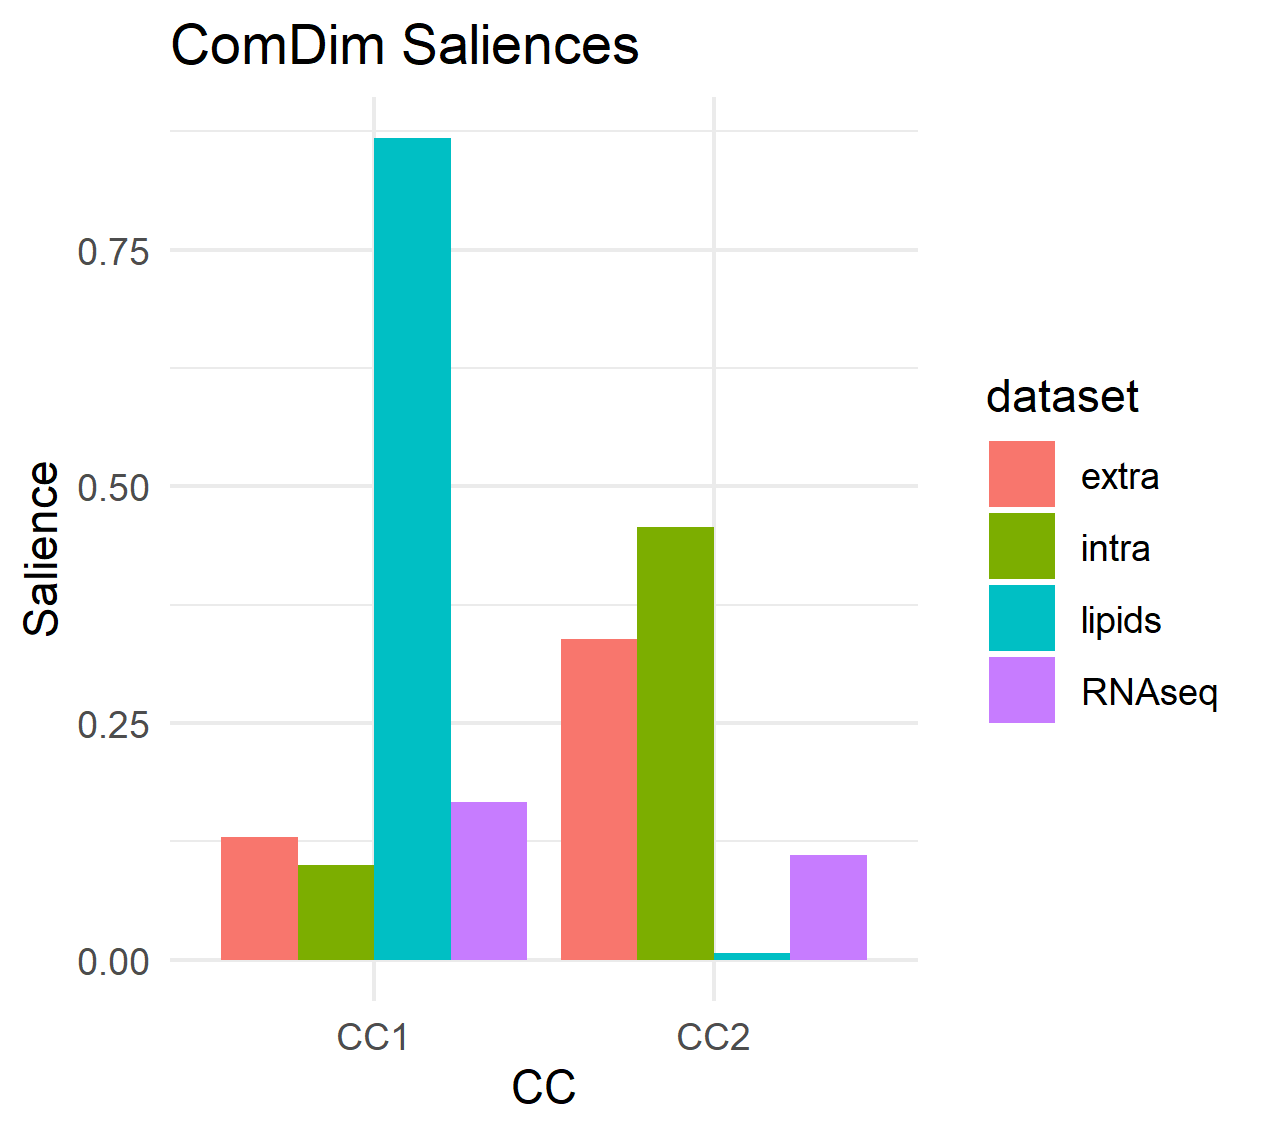
\includegraphics{Figs/fig1.png}

\hypertarget{Scores}{%
\subsection{Scores}\label{Scores}}

The scores give the contribution of each sample. There are two types of scores,
\textbf{Global} (Q.scores) and \textbf{Local} (T.scores). \textbf{Global scores} show the
contribution for the total model (all blocks) while the \textbf{Local scores} give
the contribution for each of the blocks.

\begin{Shaded}
\begin{Highlighting}[]
\NormalTok{scoresTable }\OtherTok{\textless{}{-}} \FunctionTok{MakeComDimScoresTable}\NormalTok{(}\AttributeTok{model =}\NormalTok{ resultsPCA)}

\FunctionTok{head}\NormalTok{(scoresTable) }\CommentTok{\# The 6 first rows of the scores table}

\NormalTok{scoresTable\_wider }\OtherTok{\textless{}{-}}\NormalTok{ scoresTable }\SpecialCharTok{\%\textgreater{}\%}
  \FunctionTok{mutate}\NormalTok{(}\AttributeTok{sample.type =} \FunctionTok{case\_when}\NormalTok{(}\FunctionTok{grepl}\NormalTok{(}\StringTok{\textquotesingle{}DOX\textquotesingle{}}\NormalTok{, sample.id) }\SpecialCharTok{\textasciitilde{}} \StringTok{\textquotesingle{}DOX\textquotesingle{}}\NormalTok{,}
                                 \FunctionTok{grepl}\NormalTok{(}\StringTok{\textquotesingle{}NI\textquotesingle{}}\NormalTok{, sample.id) }\SpecialCharTok{\textasciitilde{}} \StringTok{\textquotesingle{}NI\textquotesingle{}}\NormalTok{,}
                                 \FunctionTok{grepl}\NormalTok{(}\StringTok{\textquotesingle{}OFF\textquotesingle{}}\NormalTok{, sample.id) }\SpecialCharTok{\textasciitilde{}} \StringTok{\textquotesingle{}OFF\textquotesingle{}}\NormalTok{)) }\SpecialCharTok{\%\textgreater{}\%}
\NormalTok{  dplyr}\SpecialCharTok{::}\FunctionTok{select}\NormalTok{(sample.id, sample.type, block.name, scores.type.dim, value) }\SpecialCharTok{\%\textgreater{}\%}
\NormalTok{  dplyr}\SpecialCharTok{::}\FunctionTok{group\_by}\NormalTok{(sample.id, sample.type, scores.type.dim, block.name) }\SpecialCharTok{\%\textgreater{}\%}
  \FunctionTok{pivot\_wider}\NormalTok{(}\AttributeTok{names\_from =}\NormalTok{ scores.type.dim, }\AttributeTok{values\_from =}\NormalTok{ value)}

\FunctionTok{ggplot}\NormalTok{(}\AttributeTok{data =}\NormalTok{ scoresTable\_wider) }\SpecialCharTok{+}
  \FunctionTok{geom\_point}\NormalTok{(}\FunctionTok{aes}\NormalTok{(}\AttributeTok{x =}\NormalTok{ T.scores1, }\AttributeTok{y =}\NormalTok{ T.scores2, }\AttributeTok{color =}\NormalTok{ sample.type,}
                 \AttributeTok{shape =}\NormalTok{ block.name)) }\SpecialCharTok{+}
  \FunctionTok{geom\_point}\NormalTok{(}\FunctionTok{aes}\NormalTok{(}\AttributeTok{x =}\NormalTok{ Q.scores1, }\AttributeTok{y =}\NormalTok{ Q.scores2,}
                 \AttributeTok{fill =}\NormalTok{ sample.type, }\AttributeTok{shape =}\NormalTok{ block.name),}
             \AttributeTok{size =} \DecValTok{3}\NormalTok{, }\AttributeTok{shape =} \DecValTok{24}\NormalTok{, }\AttributeTok{color =} \StringTok{\textquotesingle{}black\textquotesingle{}}\NormalTok{) }\SpecialCharTok{+}
  \FunctionTok{theme\_minimal}\NormalTok{() }\SpecialCharTok{+}
  \FunctionTok{labs}\NormalTok{(}\AttributeTok{title =} \StringTok{\textquotesingle{}ComDim scores\textquotesingle{}}\NormalTok{, }\AttributeTok{x =} \StringTok{\textquotesingle{}CC1\textquotesingle{}}\NormalTok{, }\AttributeTok{y =} \StringTok{\textquotesingle{}CC2\textquotesingle{}}\NormalTok{)}
  \CommentTok{\# OFF samples are very different than DOX and NI by their lipid content.}
  \CommentTok{\# Extracellular metabolites are not very different}
\end{Highlighting}
\end{Shaded}

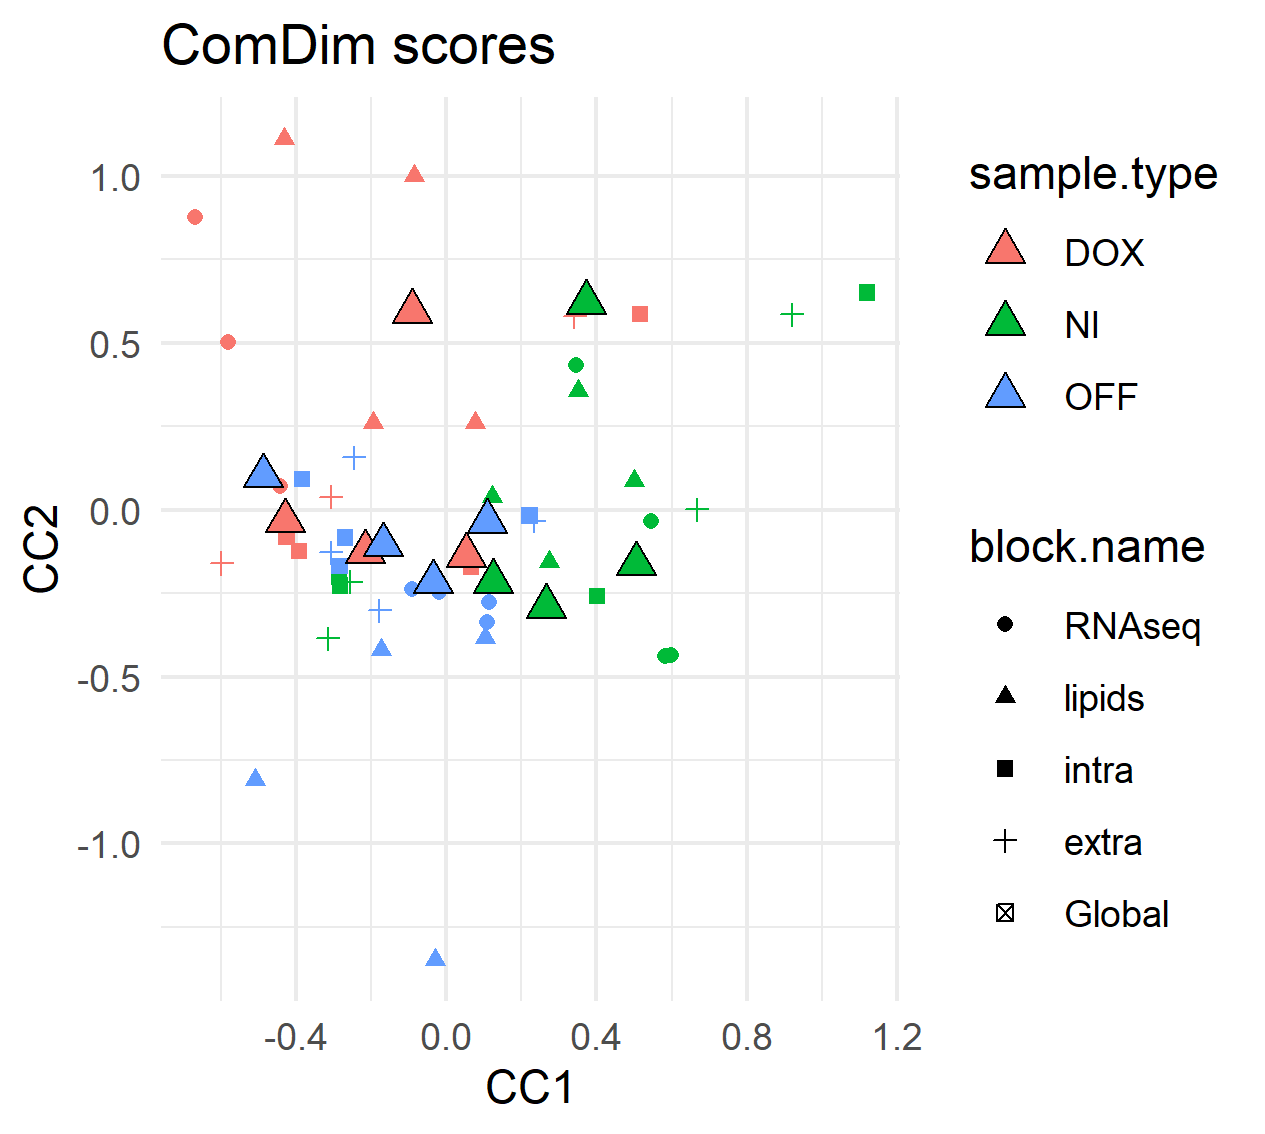
\includegraphics{Figs/fig4_2.png}

\hypertarget{Loadings}{%
\subsection{Loadings}\label{Loadings}}

The \textbf{loadings} give the contribution of each variable in the model.
And example of how to use the loadings is presented in the next section.

\hypertarget{PART3}{%
\section{Data prediction}\label{PART3}}

The built model can be used to investigate new samples if available.

\begin{Shaded}
\begin{Highlighting}[]
\NormalTok{pred.resultsPCA }\OtherTok{\textless{}{-}} \FunctionTok{Predict\_MB}\NormalTok{(}\AttributeTok{MB =}\NormalTok{ allMB, }\AttributeTok{model =}\NormalTok{ resultsPCA)}
\FunctionTok{data.frame}\NormalTok{(}\AttributeTok{original =}\NormalTok{ resultsPCA}\SpecialCharTok{@}\NormalTok{T.scores[[}\DecValTok{2}\NormalTok{]][,}\DecValTok{1}\NormalTok{],}
           \AttributeTok{predicted =}\NormalTok{ pred.resultsPCA}\SpecialCharTok{@}\NormalTok{T.scores[[}\DecValTok{2}\NormalTok{]][,}\DecValTok{1}\NormalTok{])}
\FunctionTok{data.frame}\NormalTok{(}\AttributeTok{original =}\NormalTok{ resultsPCA}\SpecialCharTok{@}\NormalTok{Q.scores[,}\DecValTok{2}\NormalTok{],}
           \AttributeTok{predicted =}\NormalTok{ resultsPCA}\SpecialCharTok{@}\NormalTok{Q.scores[,}\DecValTok{2}\NormalTok{])}
\end{Highlighting}
\end{Shaded}

In this example, the original and predicted scores are identical because the
new samples are the same as the original ones.

\hypertarget{Section5}{%
\chapter{Data from a single omics data are multi-blocks}\label{Section5}}

Metabolic pathways are composed by a group of related metabolites. Extrapolating
this concept into the MultiBlock domain, it is possible to convert a
\textbf{metabolomics dataset} into a \texttt{MultiBlock}, where each of the blocks will be
characteristic of one \textbf{metabolic pathway}.

This strategy can be applied to other types of omics datasets. For example,
\textbf{transcriptomics datasets} can be transformed to \texttt{MultiBlocks} by the
\textbf{Gene Ontology} information, and \textbf{phylogenetic data} can be split according
to any of the \textbf{taxonomic levels} (class, family, gender, species,\ldots).

In the \texttt{R.ComDim} package, this data transformation can be mediated with the
\texttt{ExpandMultiBlock()} function and a reference metadata file with the list of
categories each variable can be listed in. In the resulting \texttt{MultiBlock}, a
variable will be included in as many blocks as groups (i.e.~molecular function)
it belongs to.

\begin{Shaded}
\begin{Highlighting}[]
\FunctionTok{data}\NormalTok{(mouse\_ds)}
\NormalTok{lipidsMB }\OtherTok{\textless{}{-}} \FunctionTok{ExpandMultiBlock}\NormalTok{(}\AttributeTok{data =}\NormalTok{ lipids, }\AttributeTok{metadata =}\NormalTok{ metadata\_lipids,}
                             \AttributeTok{minblock =} \DecValTok{0}\NormalTok{, }\AttributeTok{loquace =} \ConstantTok{FALSE}\NormalTok{)}
\NormalTok{extraMB }\OtherTok{\textless{}{-}} \FunctionTok{ExpandMultiBlock}\NormalTok{(}\AttributeTok{data =}\NormalTok{ extra, }\AttributeTok{metadata =}\NormalTok{ KEGG\_table\_metabolites,}
                            \AttributeTok{minblock =} \DecValTok{10}\NormalTok{, }\AttributeTok{loquace =} \ConstantTok{FALSE}\NormalTok{)}
\NormalTok{intraMB }\OtherTok{\textless{}{-}} \FunctionTok{ExpandMultiBlock}\NormalTok{(}\AttributeTok{data =}\NormalTok{ intra, }\AttributeTok{metadata =}\NormalTok{ KEGG\_table\_metabolites,}
                            \AttributeTok{minblock =} \DecValTok{10}\NormalTok{, }\AttributeTok{loquace =} \ConstantTok{FALSE}\NormalTok{)}
\NormalTok{RNAseqMB }\OtherTok{\textless{}{-}} \FunctionTok{ExpandMultiBlock}\NormalTok{(}\AttributeTok{data =}\NormalTok{ RNAseq3[,}\DecValTok{1}\SpecialCharTok{:}\DecValTok{12}\NormalTok{],}
                             \AttributeTok{metadata =}\NormalTok{ metadata\_RNAseq3,}
                             \AttributeTok{minblock =} \DecValTok{500}\NormalTok{, }\AttributeTok{loquace =} \ConstantTok{FALSE}\NormalTok{)}
\CommentTok{\# We can count the number of blocks in each MultiBlock}
\FunctionTok{length}\NormalTok{(}\FunctionTok{getBlockNames}\NormalTok{(lipidsMB)) }\CommentTok{\# 4 blocks}
\FunctionTok{length}\NormalTok{(}\FunctionTok{getBlockNames}\NormalTok{(extraMB))  }\CommentTok{\# 12 blocks}
\FunctionTok{length}\NormalTok{(}\FunctionTok{getBlockNames}\NormalTok{(intraMB))  }\CommentTok{\# 12 blocks}
\FunctionTok{length}\NormalTok{(}\FunctionTok{getBlockNames}\NormalTok{(RNAseqMB)) }\CommentTok{\# 16 blocks}
\end{Highlighting}
\end{Shaded}

Since the blocks from this \texttt{MultiBlock} are related to a specific biological
role, the \textbf{ComDim analysis} can be used to determine the biological roles more
important in the the studied dataset.

In the \texttt{MultiBlock}s above, we only kept those blocks containing equal or more
than \texttt{minblock} variables (i.e.~only the RNAseq-related blocks containing 500 or
more variables were kept).
In order to find the most relevant pathways, ComDim will consider all blocks
equally important, causing that the variables from the smallest blocks will
contribute more to the final model than the variables from the largest blocks.
Then, the \texttt{minblock} filter is applied to avoid that the smallest blocks
(which usually relate to poorly-characterized biological roles, and thus hardly
interpretable) influence the ComDim model construction.

Let's continue with the example from before, but before the ComDim analysis we
can apply some data transformations.

\begin{Shaded}
\begin{Highlighting}[]
\CommentTok{\# Blocks are relabelled for clarity}
\NormalTok{lipidsMB }\OtherTok{\textless{}{-}} \FunctionTok{setBlockNames}\NormalTok{(lipidsMB,}
                          \FunctionTok{paste}\NormalTok{(}\StringTok{"lipids"}\NormalTok{, }\FunctionTok{getBlockNames}\NormalTok{(lipidsMB), }\AttributeTok{sep =} \StringTok{\textquotesingle{}.\textquotesingle{}}\NormalTok{))}
\NormalTok{intraMB }\OtherTok{\textless{}{-}} \FunctionTok{setBlockNames}\NormalTok{(intraMB,}
                         \FunctionTok{paste}\NormalTok{(}\StringTok{"intra"}\NormalTok{, }\FunctionTok{getBlockNames}\NormalTok{(intraMB), }\AttributeTok{sep =} \StringTok{\textquotesingle{}.\textquotesingle{}}\NormalTok{))}
\NormalTok{extraMB }\OtherTok{\textless{}{-}} \FunctionTok{setBlockNames}\NormalTok{(extraMB,}
                         \FunctionTok{paste}\NormalTok{(}\StringTok{"extra"}\NormalTok{, }\FunctionTok{getBlockNames}\NormalTok{(extraMB), }\AttributeTok{sep =} \StringTok{\textquotesingle{}.\textquotesingle{}}\NormalTok{))}
\NormalTok{RNAseqMB }\OtherTok{\textless{}{-}} \FunctionTok{setBlockNames}\NormalTok{(RNAseqMB,}
                          \FunctionTok{paste}\NormalTok{(}\StringTok{"RNAseq"}\NormalTok{, }\FunctionTok{getBlockNames}\NormalTok{(RNAseqMB), }\AttributeTok{sep =} \StringTok{\textquotesingle{}.\textquotesingle{}}\NormalTok{))}

\NormalTok{allMB2 }\OtherTok{\textless{}{-}} \FunctionTok{BuildMultiBlock}\NormalTok{(RNAseqMB, lipidsMB, intraMB, extraMB)}
\end{Highlighting}
\end{Shaded}

Now, all 4 \texttt{MultiBlock}s were merged into a single \texttt{MultiBlock}, and each block
contains a suffix denoting the omics data type.

We apply some data pre-processings:

\begin{Shaded}
\begin{Highlighting}[]
\CommentTok{\# We apply some pre{-}processings}
  \FunctionTok{library}\NormalTok{(DESeq2)}
  \CommentTok{\# Remove blocks relative to map01100}
  \CommentTok{\# (not very informative, it\textquotesingle{}s the map with all metabolic pathways)}
\NormalTok{  allMB2 }\OtherTok{\textless{}{-}} \FunctionTok{ProcessMultiBlock}\NormalTok{(allMB2,}
    \AttributeTok{blocks =} \FunctionTok{which}\NormalTok{(}\FunctionTok{grepl}\NormalTok{(}\StringTok{\textquotesingle{}map01100\textquotesingle{}}\NormalTok{, }\FunctionTok{getBlockNames}\NormalTok{(allMB2))),}
    \CommentTok{\# All blocks with map01100 are deleted, since ncol(x) is always \textgreater{} 0.}
    \AttributeTok{FUN.SelectBlocks =} \ControlFlowTok{function}\NormalTok{(x)\{}\FunctionTok{ncol}\NormalTok{(x) }\SpecialCharTok{\textless{}} \DecValTok{0}\NormalTok{\})}
  \CommentTok{\# Calculate the absolute maximum from the RNAseq data.}
\NormalTok{  maxMB }\OtherTok{\textless{}{-}} \FunctionTok{max}\NormalTok{(}\FunctionTok{MultiBlock2matrix}\NormalTok{(allMB2,}
                                 \AttributeTok{blocks =} \FunctionTok{grep}\NormalTok{(}\StringTok{\textquotesingle{}RNAseq\textquotesingle{}}\NormalTok{,}\FunctionTok{getBlockNames}\NormalTok{(allMB2))}
\NormalTok{                                 ),}
               \AttributeTok{na.rm =} \ConstantTok{TRUE}\NormalTok{)}
  \CommentTok{\# Exclude normalized variables with max intensity reported below 0.1\%}
  \CommentTok{\# of the max from all RNAseq blocks.}
\NormalTok{  allMB2 }\OtherTok{\textless{}{-}} \FunctionTok{ProcessMultiBlock}\NormalTok{(allMB2,}
     \AttributeTok{blocks =} \FunctionTok{grep}\NormalTok{(}\StringTok{\textquotesingle{}RNAseq\textquotesingle{}}\NormalTok{,}\FunctionTok{getBlockNames}\NormalTok{(allMB2)),}
     \AttributeTok{FUN.SelectVars =} \ControlFlowTok{function}\NormalTok{(x) \{}\FunctionTok{apply}\NormalTok{(x,}\DecValTok{2}\NormalTok{,max) }\SpecialCharTok{\textgreater{}}\NormalTok{ maxMB }\SpecialCharTok{*} \FloatTok{0.001}\NormalTok{\})}
  \CommentTok{\# Add 1 to each value in RNAseq data to remove 0s.}
\NormalTok{  allMB2 }\OtherTok{\textless{}{-}} \FunctionTok{NARemoveMultiBlock}\NormalTok{(allMB2,}
     \AttributeTok{blocks =} \FunctionTok{grep}\NormalTok{(}\StringTok{\textquotesingle{}RNAseq\textquotesingle{}}\NormalTok{,}\FunctionTok{getBlockNames}\NormalTok{(allMB2)),}
     \AttributeTok{method =} \StringTok{\textquotesingle{}fixed.value.all\textquotesingle{}}\NormalTok{,}
     \AttributeTok{constant =} \DecValTok{1}\NormalTok{)}
  \CommentTok{\# Do rlog transform of the RNAseq data.}
\NormalTok{  allMB2 }\OtherTok{\textless{}{-}} \FunctionTok{ProcessMultiBlock}\NormalTok{(allMB2,}
     \AttributeTok{blocks =} \FunctionTok{grep}\NormalTok{(}\StringTok{\textquotesingle{}RNAseq\textquotesingle{}}\NormalTok{,}\FunctionTok{getBlockNames}\NormalTok{(allMB2)),}
     \CommentTok{\# Normalize rlog transcript counts}
     \AttributeTok{FUN =} \ControlFlowTok{function}\NormalTok{(x)\{}\FunctionTok{t}\NormalTok{(DESeq2}\SpecialCharTok{::}\FunctionTok{rlog}\NormalTok{(}\FunctionTok{t}\NormalTok{(x)))\})}
  \CommentTok{\# Replace NAs by random noise}
\NormalTok{  allMB2 }\OtherTok{\textless{}{-}} \FunctionTok{NARemoveMultiBlock}\NormalTok{(allMB2, }\AttributeTok{method =} \StringTok{\textquotesingle{}random.noise\textquotesingle{}}\NormalTok{)}
  \CommentTok{\# Normalize (mean{-}center and divided by each block{-}norm)}
\NormalTok{  allMB2 }\OtherTok{\textless{}{-}} \FunctionTok{NormalizeMultiBlock}\NormalTok{(allMB2, }\AttributeTok{method =} \StringTok{\textquotesingle{}norm\textquotesingle{}}\NormalTok{)}
\end{Highlighting}
\end{Shaded}

We continue with the ComDim analysis:

\begin{Shaded}
\begin{Highlighting}[]
\NormalTok{  resultsPCA2 }\OtherTok{\textless{}{-}} \FunctionTok{ComDim\_PCA\_MB}\NormalTok{(allMB2, }\AttributeTok{ndim =} \DecValTok{2}\NormalTok{)}
\end{Highlighting}
\end{Shaded}

A first look at the scores can tell us how the blocks relate to the sample type.

\begin{Shaded}
\begin{Highlighting}[]
\NormalTok{  scoresTable }\OtherTok{\textless{}{-}} \FunctionTok{MakeComDimScoresTable}\NormalTok{(}\AttributeTok{model =}\NormalTok{ resultsPCA2)}
\NormalTok{  scoresTable\_wider }\OtherTok{\textless{}{-}}\NormalTok{ scoresTable }\SpecialCharTok{\%\textgreater{}\%}
    \FunctionTok{mutate}\NormalTok{(}\AttributeTok{sample.type =} \FunctionTok{case\_when}\NormalTok{(}\FunctionTok{grepl}\NormalTok{(}\StringTok{\textquotesingle{}DOX\textquotesingle{}}\NormalTok{, sample.id) }\SpecialCharTok{\textasciitilde{}} \StringTok{\textquotesingle{}DOX\textquotesingle{}}\NormalTok{,}
                                   \FunctionTok{grepl}\NormalTok{(}\StringTok{\textquotesingle{}NI\textquotesingle{}}\NormalTok{, sample.id) }\SpecialCharTok{\textasciitilde{}} \StringTok{\textquotesingle{}NI\textquotesingle{}}\NormalTok{,}
                                   \FunctionTok{grepl}\NormalTok{(}\StringTok{\textquotesingle{}OFF\textquotesingle{}}\NormalTok{, sample.id) }\SpecialCharTok{\textasciitilde{}} \StringTok{\textquotesingle{}OFF\textquotesingle{}}\NormalTok{)) }\SpecialCharTok{\%\textgreater{}\%}
\NormalTok{    dplyr}\SpecialCharTok{::}\FunctionTok{select}\NormalTok{(sample.id, sample.type, block.name, scores.type.dim, value) }\SpecialCharTok{\%\textgreater{}\%}
\NormalTok{    dplyr}\SpecialCharTok{::}\FunctionTok{group\_by}\NormalTok{(sample.id, sample.type, scores.type.dim, block.name) }\SpecialCharTok{\%\textgreater{}\%}
    \FunctionTok{pivot\_wider}\NormalTok{(}\AttributeTok{names\_from =}\NormalTok{ scores.type.dim, }\AttributeTok{values\_from =}\NormalTok{ value) }\SpecialCharTok{\%\textgreater{}\%}
    \FunctionTok{mutate}\NormalTok{(}\AttributeTok{omics =} \FunctionTok{case\_when}\NormalTok{(}\FunctionTok{grepl}\NormalTok{(}\StringTok{\textquotesingle{}RNAseq\textquotesingle{}}\NormalTok{, block.name) }\SpecialCharTok{\textasciitilde{}} \StringTok{\textquotesingle{}RNAseq\textquotesingle{}}\NormalTok{,}
                             \FunctionTok{grepl}\NormalTok{(}\StringTok{\textquotesingle{}lipids\textquotesingle{}}\NormalTok{, block.name) }\SpecialCharTok{\textasciitilde{}} \StringTok{\textquotesingle{}lipids\textquotesingle{}}\NormalTok{,}
                             \FunctionTok{grepl}\NormalTok{(}\StringTok{\textquotesingle{}extra\textquotesingle{}}\NormalTok{, block.name) }\SpecialCharTok{\textasciitilde{}} \StringTok{\textquotesingle{}extra\textquotesingle{}}\NormalTok{,}
                             \FunctionTok{grepl}\NormalTok{(}\StringTok{\textquotesingle{}intra\textquotesingle{}}\NormalTok{, block.name) }\SpecialCharTok{\textasciitilde{}} \StringTok{\textquotesingle{}intra\textquotesingle{}}\NormalTok{,}
                             \FunctionTok{grepl}\NormalTok{(}\StringTok{\textquotesingle{}Global\textquotesingle{}}\NormalTok{, block.name) }\SpecialCharTok{\textasciitilde{}} \StringTok{\textquotesingle{}Global\textquotesingle{}}\NormalTok{))}

  \FunctionTok{ggplot}\NormalTok{(}\AttributeTok{data =}\NormalTok{ scoresTable\_wider) }\SpecialCharTok{+}
    \FunctionTok{geom\_point}\NormalTok{(}\FunctionTok{aes}\NormalTok{(}\AttributeTok{x =}\NormalTok{ T.scores1, }\AttributeTok{y =}\NormalTok{ T.scores2, }\AttributeTok{color =}\NormalTok{ sample.type, }\AttributeTok{shape =}\NormalTok{ omics)) }\SpecialCharTok{+}
    \FunctionTok{geom\_point}\NormalTok{(}\FunctionTok{aes}\NormalTok{(}\AttributeTok{x =}\NormalTok{ Q.scores1, }\AttributeTok{y =}\NormalTok{ Q.scores2, }\AttributeTok{fill =}\NormalTok{ sample.type),}
               \AttributeTok{size =} \DecValTok{3}\NormalTok{, }\AttributeTok{shape =} \DecValTok{24}\NormalTok{, }\AttributeTok{color =} \StringTok{\textquotesingle{}black\textquotesingle{}}\NormalTok{) }\SpecialCharTok{+}
    \FunctionTok{theme\_minimal}\NormalTok{() }\SpecialCharTok{+}
    \FunctionTok{labs}\NormalTok{(}\AttributeTok{title =} \StringTok{\textquotesingle{}ComDim scores\textquotesingle{}}\NormalTok{, }\AttributeTok{x =} \StringTok{\textquotesingle{}CC1\textquotesingle{}}\NormalTok{, }\AttributeTok{y =} \StringTok{\textquotesingle{}CC2\textquotesingle{}}\NormalTok{)}
\end{Highlighting}
\end{Shaded}

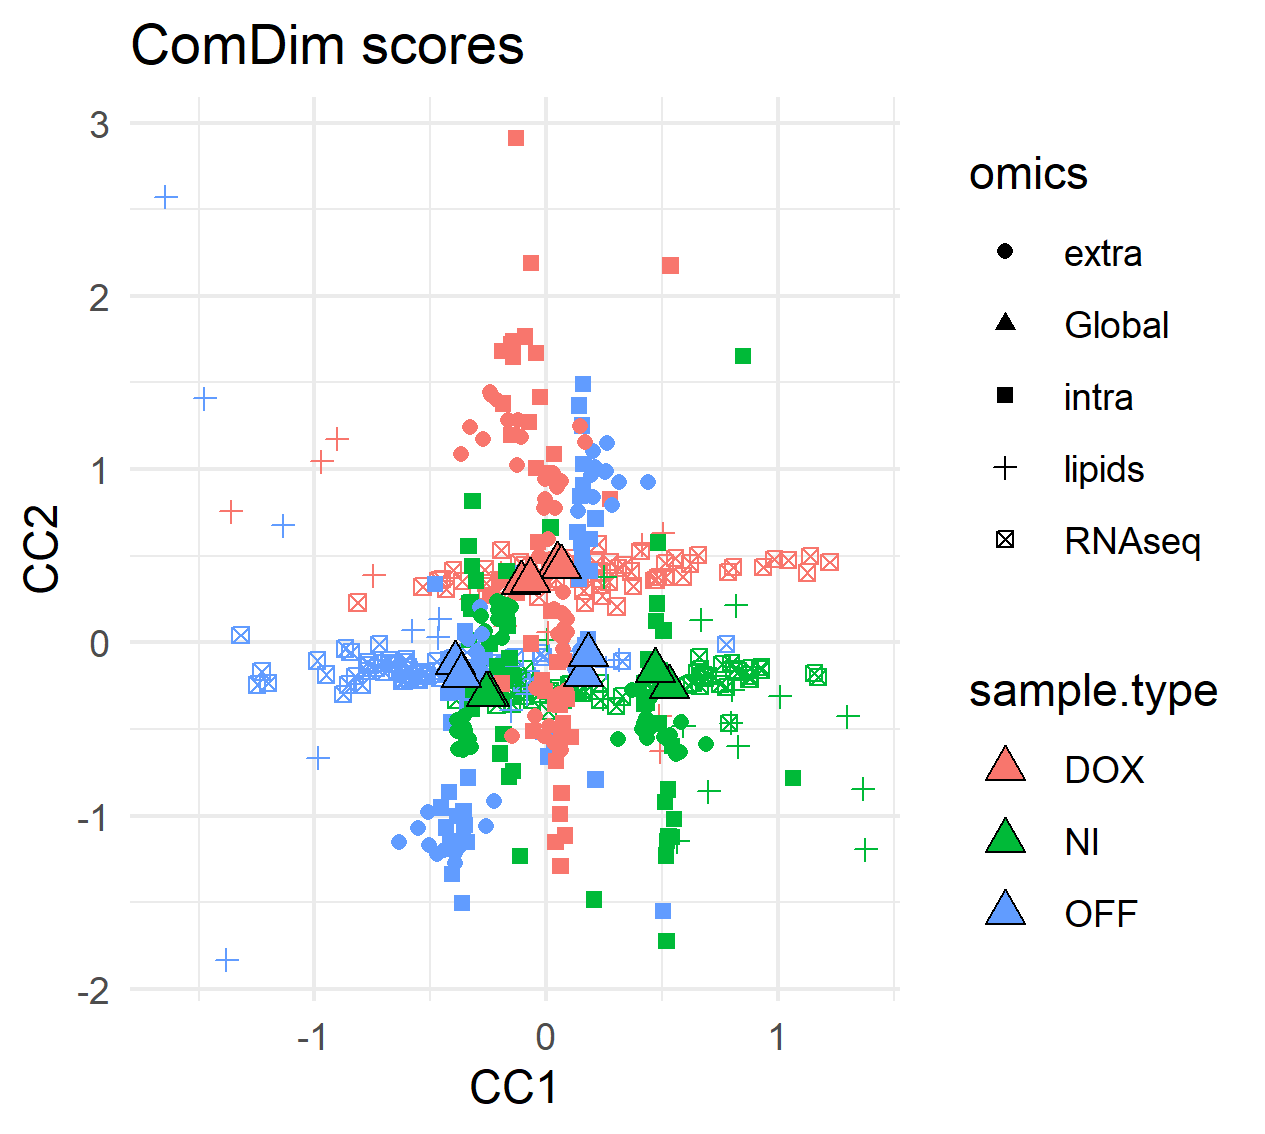
\includegraphics{Figs/fig5_1.png}

The metabolomic and the RNAseq profiles appear to be very orthogonal
(uncorrelated), since intra and extra does not change much (within each group)
in CC2 whereas the RNAseq does not change much in CC1.
For RNAseq molecular functions, CC1 separates OFF from NI and DOX.
CC2 separates DOX from NI and OFF.
Despite this, NI seems to be different from DOX and OFF at the lipidomic level.

\hypertarget{molecular-functions}{%
\section{Molecular functions}\label{molecular-functions}}

Let's start by looking at the \textbf{saliences}:

\begin{Shaded}
\begin{Highlighting}[]
\CommentTok{\# Plot saliences}
\NormalTok{saliences2 }\OtherTok{\textless{}{-}}\NormalTok{ resultsPCA2}\SpecialCharTok{@}\NormalTok{Saliences }\SpecialCharTok{\%\textgreater{}\%}
  \FunctionTok{as.data.frame}\NormalTok{() }\SpecialCharTok{\%\textgreater{}\%}
  \FunctionTok{mutate}\NormalTok{(}\AttributeTok{dataset =} \FunctionTok{rownames}\NormalTok{(.)) }\SpecialCharTok{\%\textgreater{}\%}
  \FunctionTok{pivot\_longer}\NormalTok{(}\AttributeTok{cols =} \FunctionTok{c}\NormalTok{(}\StringTok{\textquotesingle{}CC1\textquotesingle{}}\NormalTok{,}\StringTok{\textquotesingle{}CC2\textquotesingle{}}\NormalTok{),}
               \AttributeTok{names\_to =} \StringTok{\textquotesingle{}CC\textquotesingle{}}\NormalTok{,}
               \AttributeTok{values\_to =} \StringTok{\textquotesingle{}Salience\textquotesingle{}}\NormalTok{) }\SpecialCharTok{\%\textgreater{}\%}
  \FunctionTok{mutate}\NormalTok{(}\AttributeTok{omics =} \FunctionTok{case\_when}\NormalTok{(}\FunctionTok{grepl}\NormalTok{(}\StringTok{\textquotesingle{}RNAseq\textquotesingle{}}\NormalTok{, dataset) }\SpecialCharTok{\textasciitilde{}} \StringTok{\textquotesingle{}RNAseq\textquotesingle{}}\NormalTok{,}
                           \FunctionTok{grepl}\NormalTok{(}\StringTok{\textquotesingle{}lipids\textquotesingle{}}\NormalTok{, dataset) }\SpecialCharTok{\textasciitilde{}} \StringTok{\textquotesingle{}lipids\textquotesingle{}}\NormalTok{,}
                           \FunctionTok{grepl}\NormalTok{(}\StringTok{\textquotesingle{}extra\textquotesingle{}}\NormalTok{, dataset) }\SpecialCharTok{\textasciitilde{}} \StringTok{\textquotesingle{}extra\textquotesingle{}}\NormalTok{,}
                           \FunctionTok{grepl}\NormalTok{(}\StringTok{\textquotesingle{}intra\textquotesingle{}}\NormalTok{, dataset) }\SpecialCharTok{\textasciitilde{}} \StringTok{\textquotesingle{}intra\textquotesingle{}}\NormalTok{))}
  \FunctionTok{ggplot}\NormalTok{(}\AttributeTok{data =}\NormalTok{ saliences2,}
       \FunctionTok{aes}\NormalTok{(}\AttributeTok{x =}\NormalTok{ CC, }\AttributeTok{y =}\NormalTok{ Salience, }\AttributeTok{group =}\NormalTok{ dataset )) }\SpecialCharTok{+}
  \FunctionTok{geom\_bar}\NormalTok{(}\AttributeTok{stat =} \StringTok{\textquotesingle{}identity\textquotesingle{}}\NormalTok{, }\AttributeTok{position =} \StringTok{\textquotesingle{}dodge\textquotesingle{}}\NormalTok{,}
           \FunctionTok{aes}\NormalTok{(}\AttributeTok{fill =}\NormalTok{ omics)) }\SpecialCharTok{+}
  \FunctionTok{theme\_minimal}\NormalTok{() }\SpecialCharTok{+}
  \FunctionTok{geom\_text}\NormalTok{(}\AttributeTok{label =} \StringTok{\textquotesingle{}lipids.GLP\textquotesingle{}}\NormalTok{, }\AttributeTok{x =} \DecValTok{2}\NormalTok{, }\AttributeTok{y =} \FloatTok{0.4}\NormalTok{, }\AttributeTok{size =} \DecValTok{3}\NormalTok{) }\SpecialCharTok{+}
  \FunctionTok{geom\_text}\NormalTok{(}\AttributeTok{label =} \StringTok{\textquotesingle{}intra.map04978\textquotesingle{}}\NormalTok{, }\AttributeTok{x =} \FloatTok{1.25}\NormalTok{, }\AttributeTok{y =} \FloatTok{0.88}\NormalTok{, }\AttributeTok{size =} \DecValTok{3}\NormalTok{) }\SpecialCharTok{+}
  \FunctionTok{labs}\NormalTok{(}\AttributeTok{title =} \StringTok{\textquotesingle{}ComDim Saliences\textquotesingle{}}\NormalTok{)}
\end{Highlighting}
\end{Shaded}

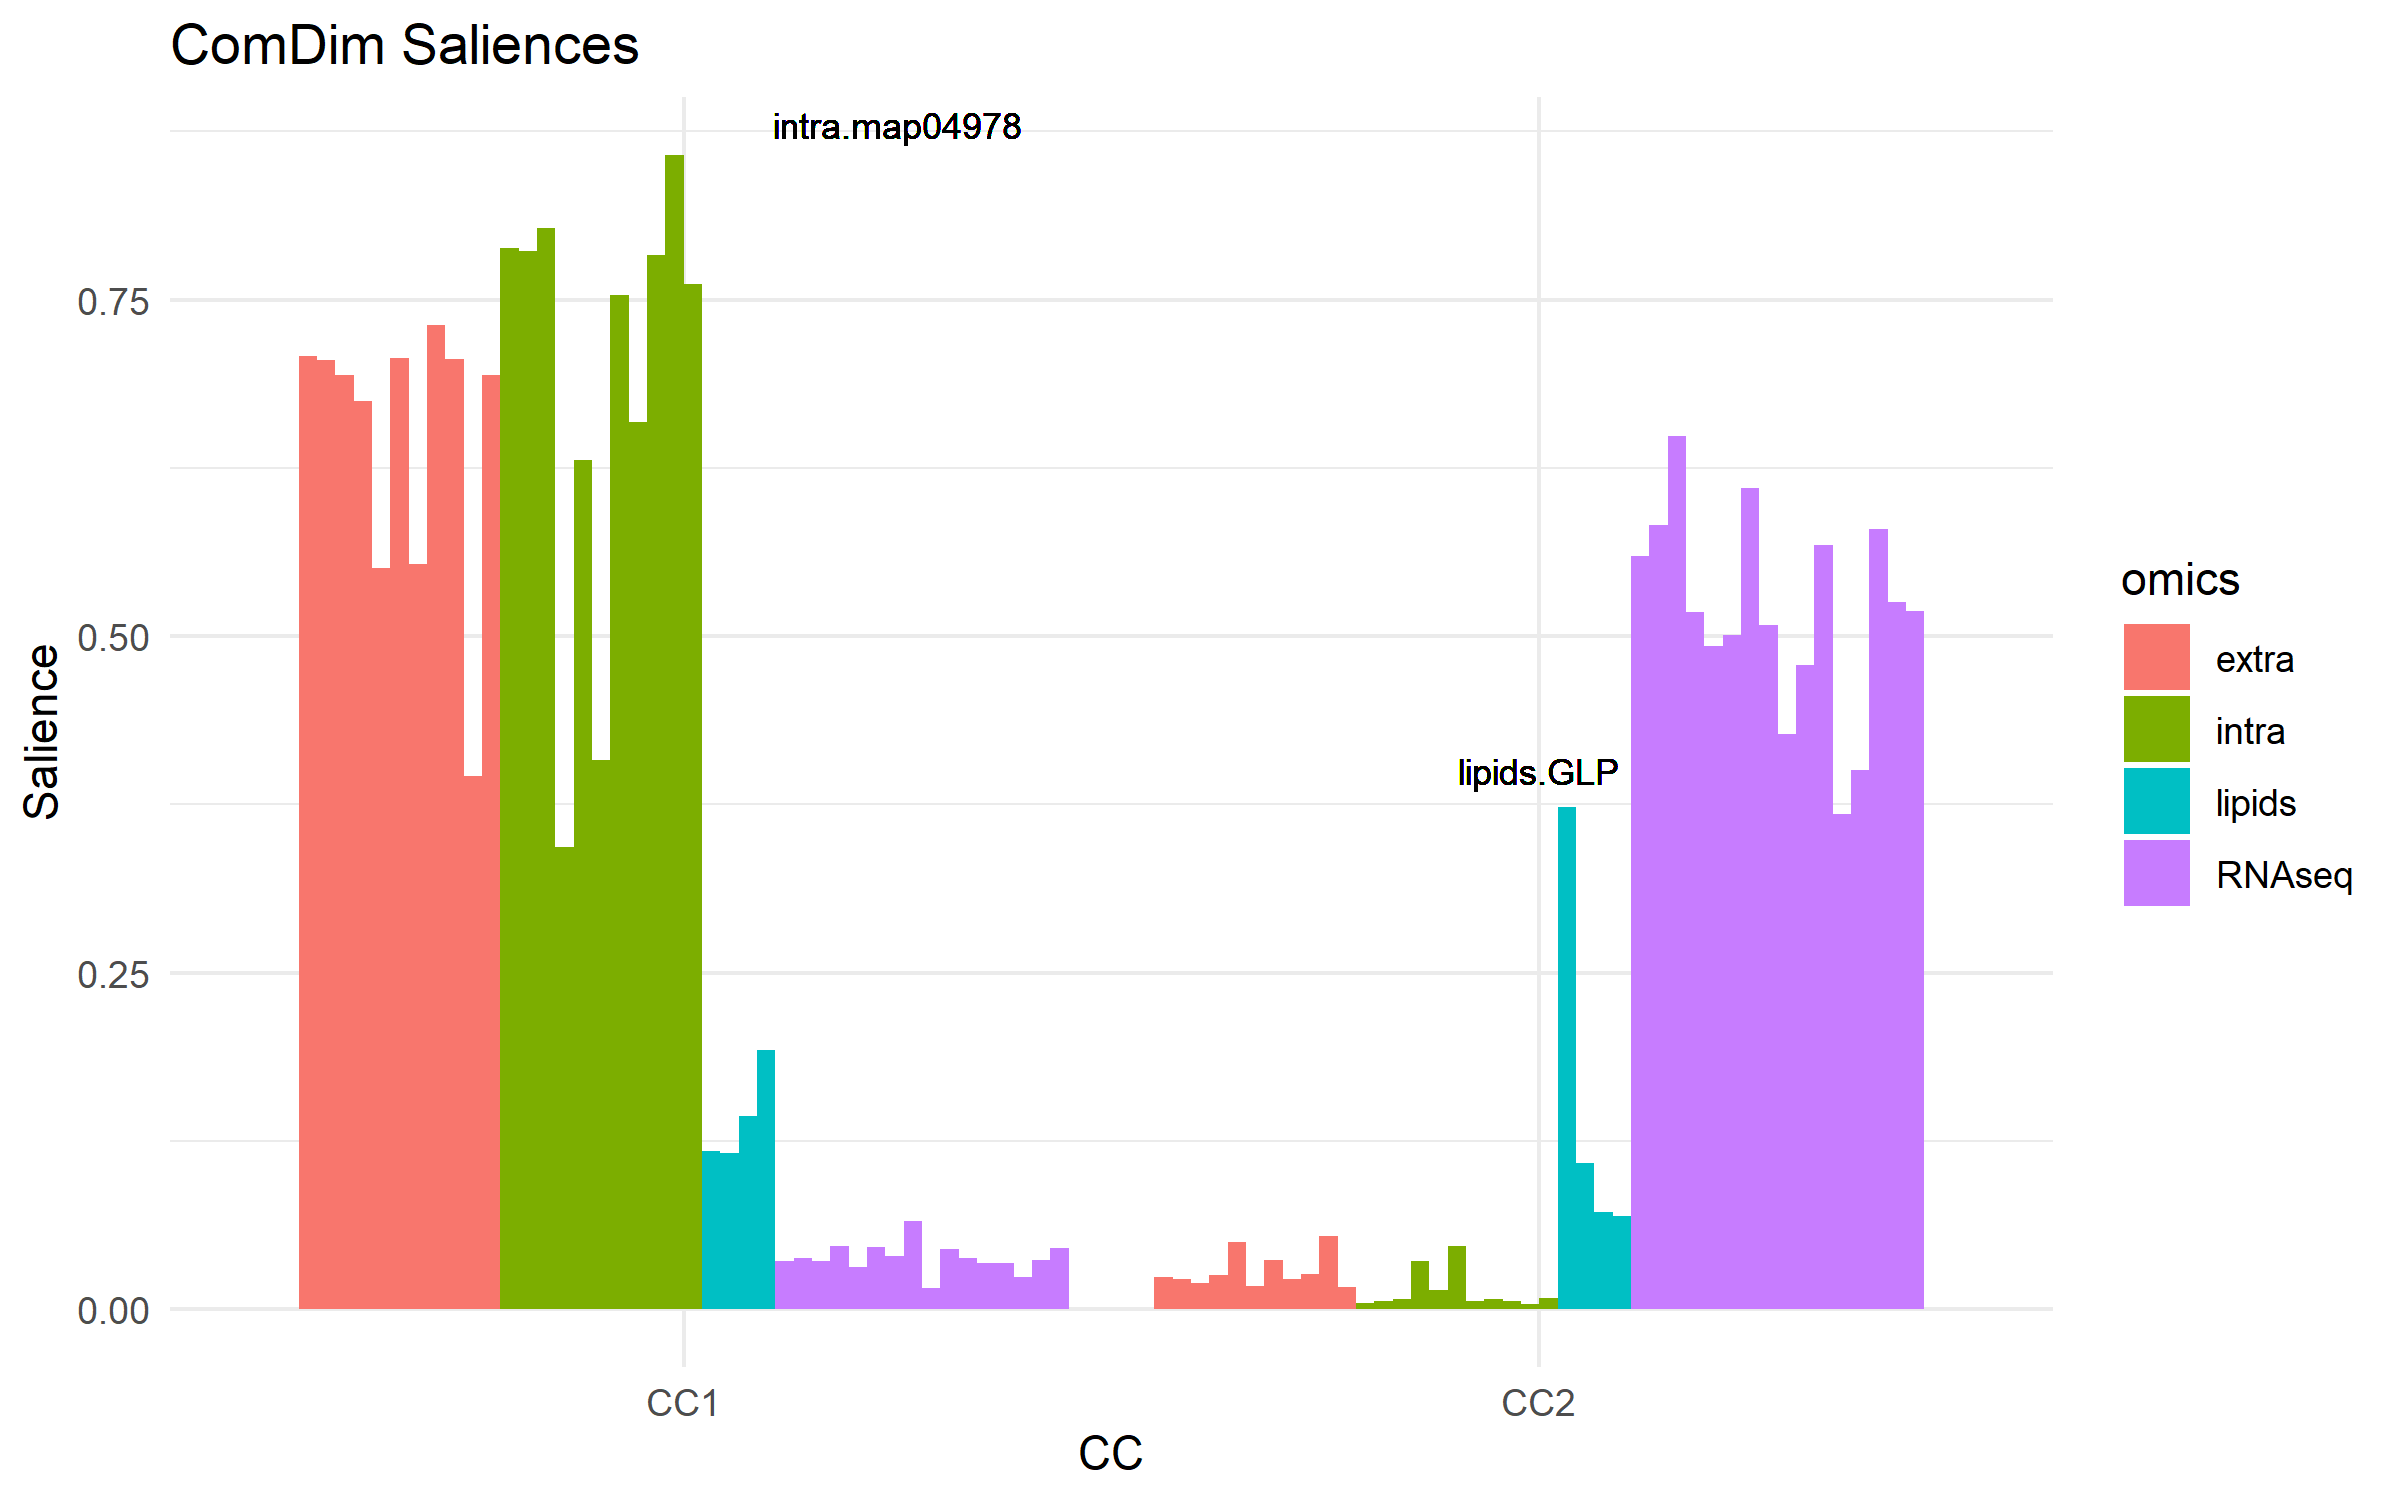
\includegraphics{Figs/fig5_2.png}
CC1 is descriptive of metabolomics data (both intra and extra)
CC2 is descriptive of RNAseq and glycerophospholipids (lipids.GLP)
The most altered molecular function is map04978 (mineral absorption),
in the ``intra'' data.

\hypertarget{the-molecular-patwhays}{%
\subsection{The molecular patwhays}\label{the-molecular-patwhays}}

By inspecting the loadings, we can have an idea of the most altered omics
features in the block.
We will plot now the loadings for the two most relevant blocks as seen in the
previous section.

\begin{Shaded}
\begin{Highlighting}[]
  \CommentTok{\# MINERAL ABSORPTION}
\NormalTok{  LoadingsTable }\OtherTok{\textless{}{-}} \FunctionTok{MakeComDimLoadingsTable}\NormalTok{(}\AttributeTok{model =}\NormalTok{ resultsPCA2,}
                                           \AttributeTok{block =} \StringTok{\textquotesingle{}intra.map04978\textquotesingle{}}\NormalTok{,}
                                           \AttributeTok{dim =} \DecValTok{1}\NormalTok{)}
  \FunctionTok{ggplot}\NormalTok{(LoadingsTable, }\FunctionTok{aes}\NormalTok{(}\AttributeTok{x =}\NormalTok{ variable.id, }\AttributeTok{y =}\NormalTok{ value)) }\SpecialCharTok{+}
    \FunctionTok{geom\_bar}\NormalTok{(}\AttributeTok{stat =} \StringTok{\textquotesingle{}identity\textquotesingle{}}\NormalTok{) }\SpecialCharTok{+}
    \FunctionTok{labs}\NormalTok{(}\AttributeTok{title =} \StringTok{\textquotesingle{}MINERAL ABSORPTION\textquotesingle{}}\NormalTok{) }\SpecialCharTok{+}
    \FunctionTok{theme\_minimal}\NormalTok{() }\SpecialCharTok{+}
    \FunctionTok{theme}\NormalTok{(}\AttributeTok{axis.text.x =} \FunctionTok{element\_text}\NormalTok{(}\AttributeTok{angle =} \DecValTok{90}\NormalTok{, }\AttributeTok{vjust =} \FloatTok{0.5}\NormalTok{, }\AttributeTok{hjust=}\DecValTok{1}\NormalTok{))}

  \CommentTok{\# GLYCEROPHOSPHOLIPIDS}
\NormalTok{  LoadingsTable }\OtherTok{\textless{}{-}} \FunctionTok{MakeComDimLoadingsTable}\NormalTok{(}\AttributeTok{model =}\NormalTok{ resultsPCA2,}
                                           \AttributeTok{block =} \StringTok{\textquotesingle{}lipids.GPL\textquotesingle{}}\NormalTok{,}
                                           \AttributeTok{dim =} \DecValTok{2}\NormalTok{)}
  \FunctionTok{ggplot}\NormalTok{(LoadingsTable, }\FunctionTok{aes}\NormalTok{(}\AttributeTok{x =}\NormalTok{ variable.id, }\AttributeTok{y =}\NormalTok{ value)) }\SpecialCharTok{+}
    \FunctionTok{geom\_bar}\NormalTok{(}\AttributeTok{stat =} \StringTok{\textquotesingle{}identity\textquotesingle{}}\NormalTok{) }\SpecialCharTok{+}
        \FunctionTok{labs}\NormalTok{(}\AttributeTok{title =} \StringTok{\textquotesingle{}GLYCEROPHOSPHOLIPIDS\textquotesingle{}}\NormalTok{) }\SpecialCharTok{+}
    \FunctionTok{theme\_minimal}\NormalTok{() }\SpecialCharTok{+}
    \FunctionTok{theme}\NormalTok{(}\AttributeTok{axis.text.x =} \FunctionTok{element\_text}\NormalTok{(}\AttributeTok{angle =} \DecValTok{90}\NormalTok{, }\AttributeTok{vjust =} \FloatTok{0.5}\NormalTok{, }\AttributeTok{hjust=}\DecValTok{1}\NormalTok{,}
                                     \AttributeTok{size =} \DecValTok{3}\NormalTok{))}
\end{Highlighting}
\end{Shaded}

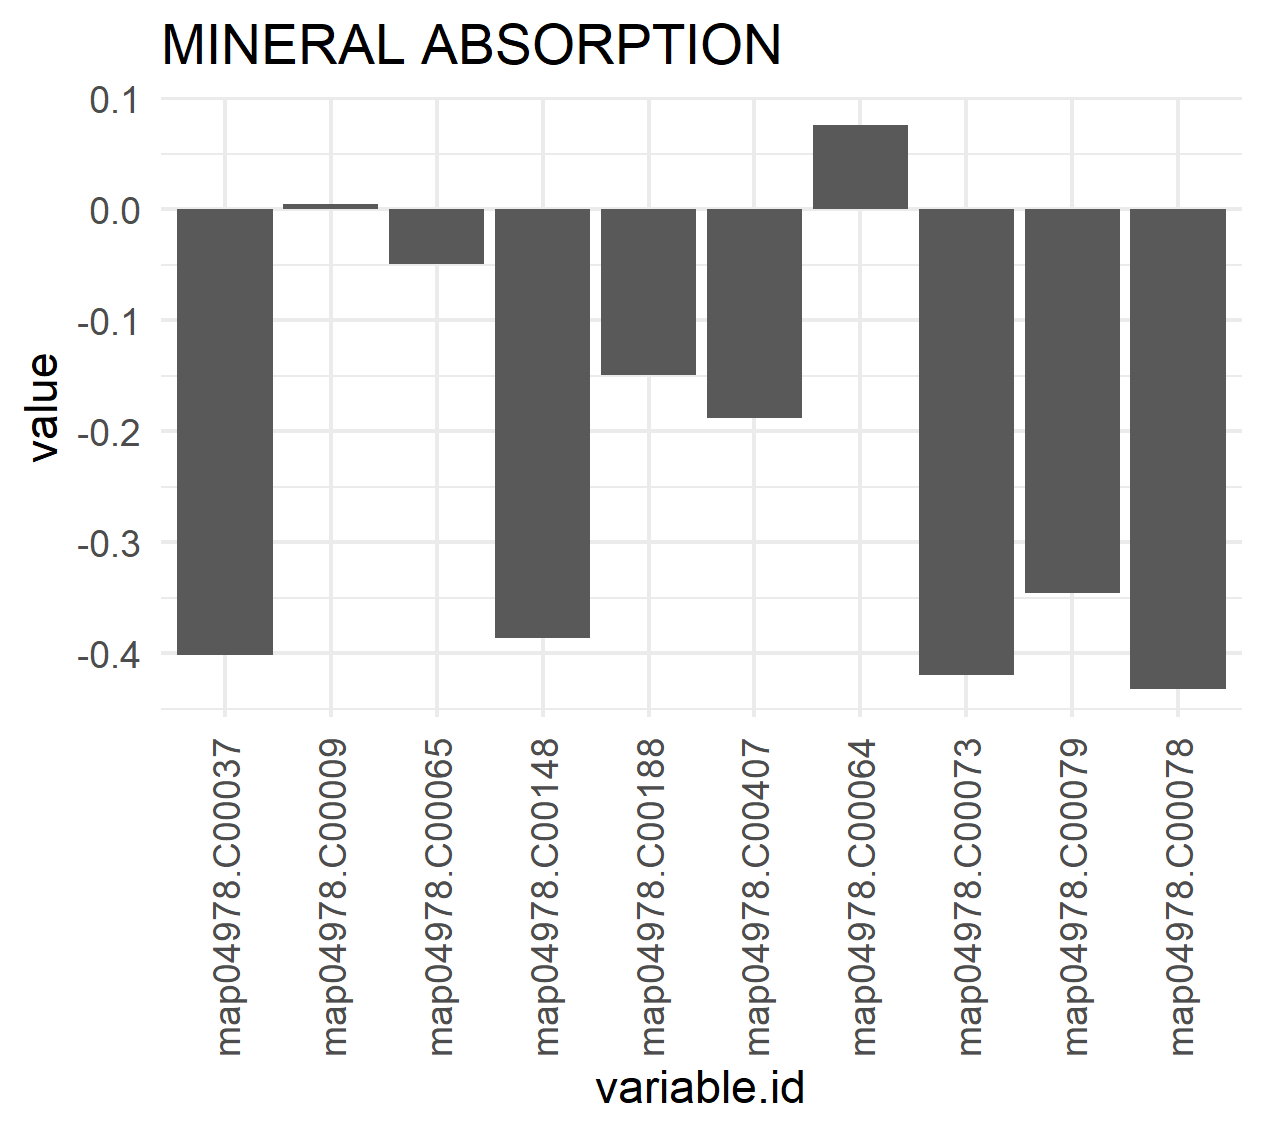
\includegraphics{Figs/fig5_3.png}
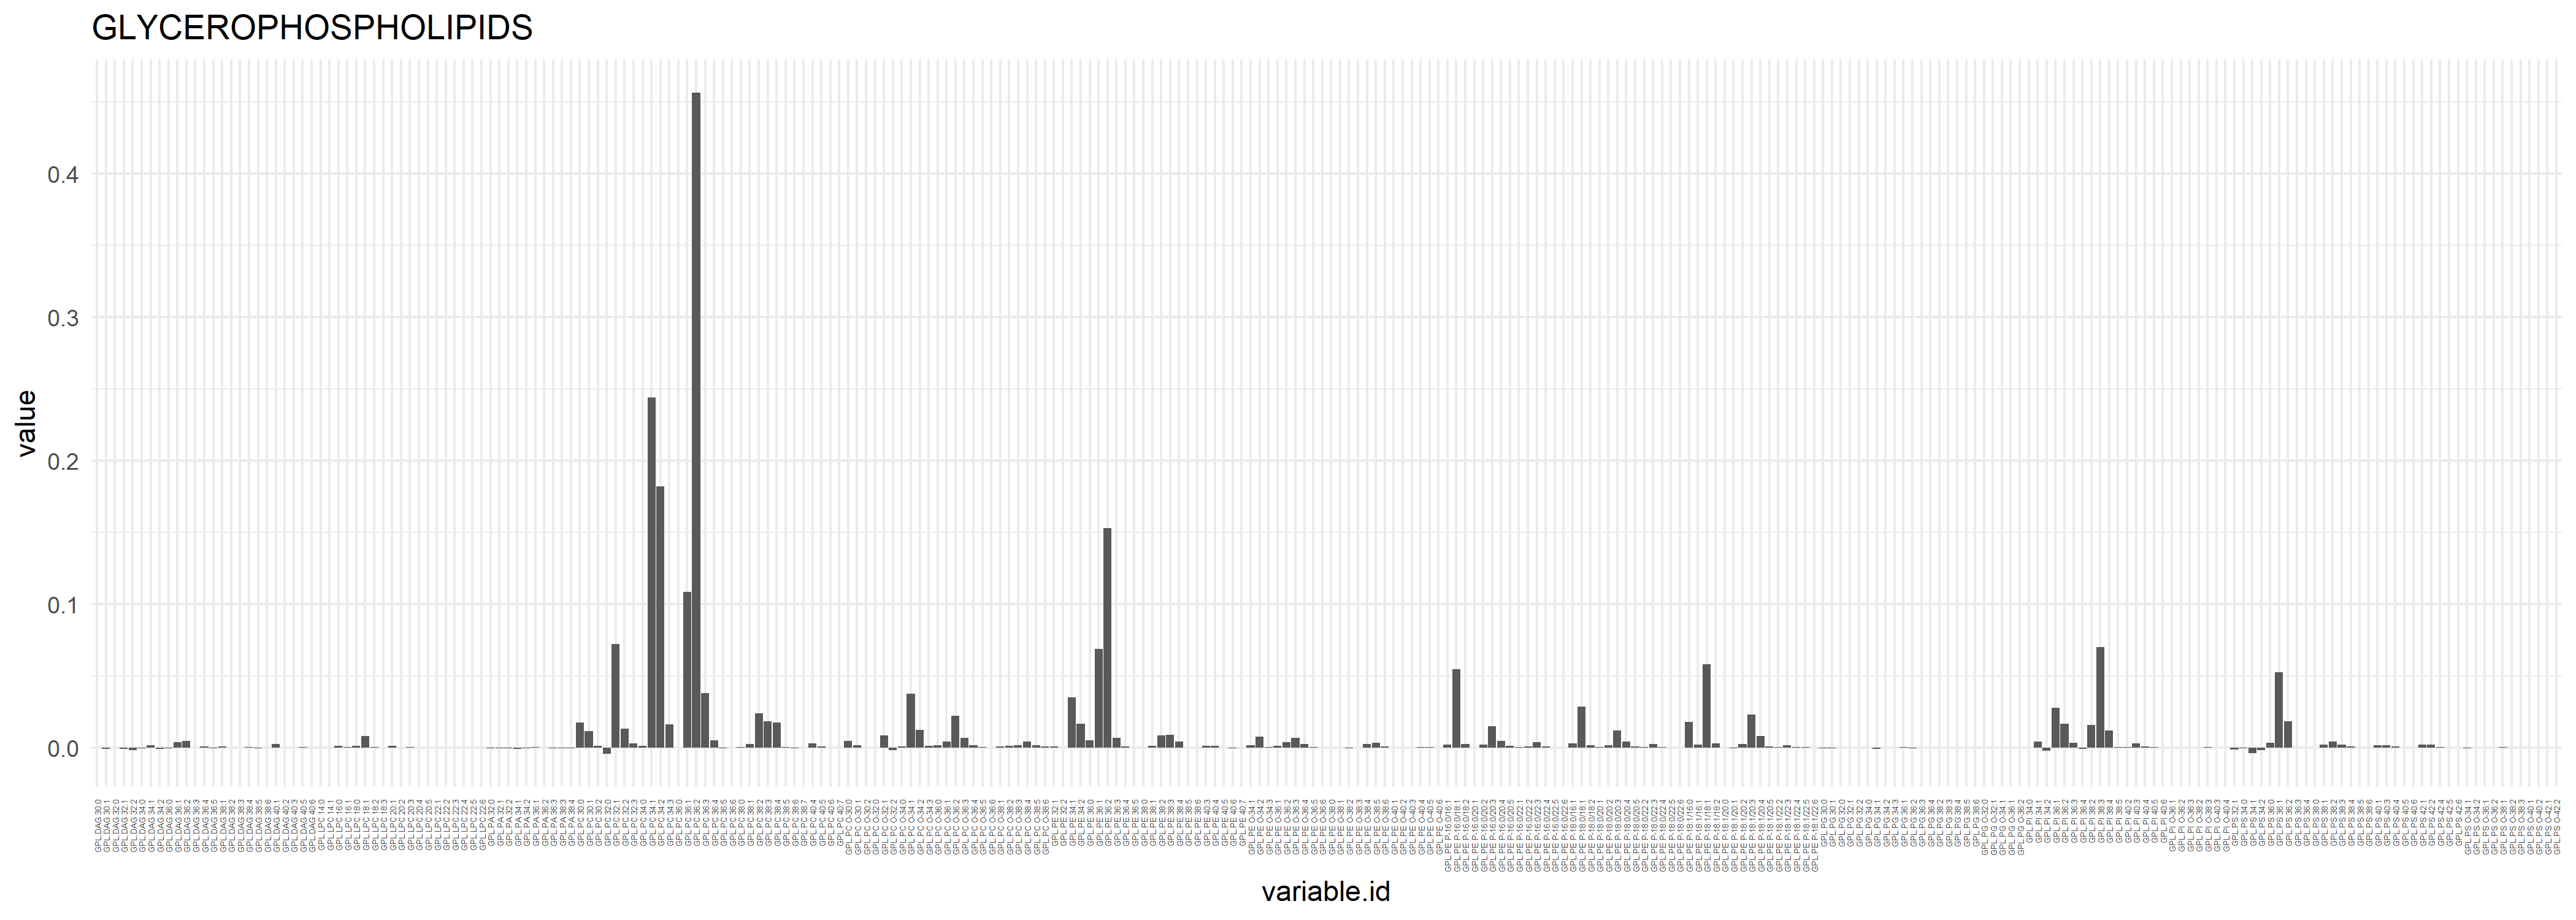
\includegraphics{Figs/fig5_4.png}
Most important changes in the GPL group occur for PC36:2, PC34:1, PC:34:2,
PE36:2, PC36:1,\ldots{}

We can also plot the loadings into \textbf{KEGG pathway maps} (if the omics variables
can be matched with the KEGG identifiers).

Here is an example for the metabolomics data:

\begin{Shaded}
\begin{Highlighting}[]
\CommentTok{\# MINERAL ABSORPTION}
\CommentTok{\# Prepare input data}
\NormalTok{loadingVector }\OtherTok{\textless{}{-}}\NormalTok{ LoadingsTable}\SpecialCharTok{$}\NormalTok{value }\SpecialCharTok{*} \DecValTok{10} \CommentTok{\# 10 is a factor used to maximize}
                                          \CommentTok{\# the color contrast in the resulting}
                                          \CommentTok{\# KEGG map.}
\FunctionTok{names}\NormalTok{(loadingVector) }\OtherTok{\textless{}{-}} \FunctionTok{gsub}\NormalTok{(}\StringTok{"map04978."}\NormalTok{,}\StringTok{""}\NormalTok{,LoadingsTable}\SpecialCharTok{$}\NormalTok{variable.id)}

\FunctionTok{library}\NormalTok{(pathview) }\CommentTok{\# From Bioconductor}
\NormalTok{pv.out }\OtherTok{\textless{}{-}} \FunctionTok{pathview}\NormalTok{(}\AttributeTok{cpd.data =}\NormalTok{ loadingVector,}
                   \AttributeTok{pathway.id =} \StringTok{"04978"}\NormalTok{,}
                   \AttributeTok{species =} \StringTok{"mmu"}\NormalTok{,}
                   \AttributeTok{out.suffix =} \StringTok{"ComDim"}\NormalTok{)}
\end{Highlighting}
\end{Shaded}

The map is saved in the working directory:
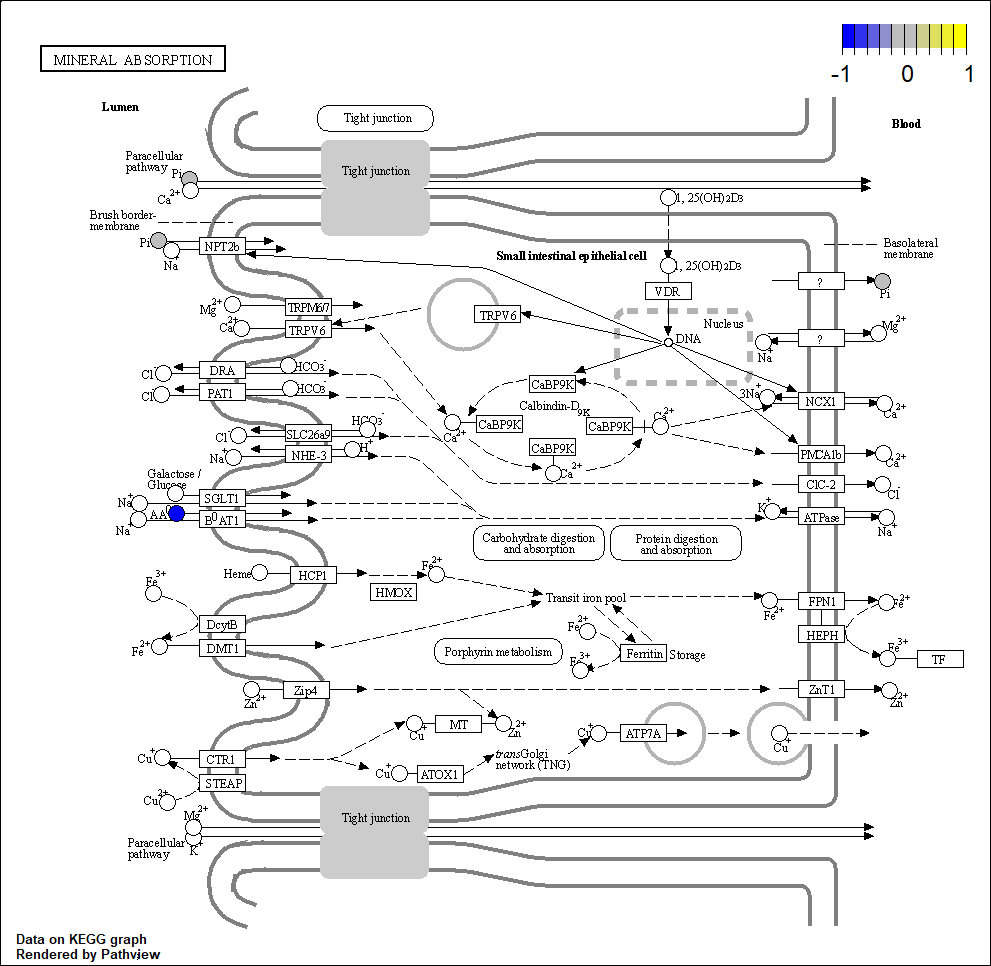
\includegraphics{Figs/mmu04978.ComDim.png}

And here, there is an example for the RNAseq-data (block mmu05200, ``Pathways in
Cancer''):

\begin{Shaded}
\begin{Highlighting}[]
\NormalTok{LoadingsTable }\OtherTok{\textless{}{-}} \FunctionTok{MakeComDimLoadingsTable}\NormalTok{(}\AttributeTok{model =}\NormalTok{ resultsPCA2,}
                                           \AttributeTok{block =} \StringTok{\textquotesingle{}RNAseq.mmu05200\textquotesingle{}}\NormalTok{,}
                                           \AttributeTok{dim =} \DecValTok{2}\NormalTok{)}
\CommentTok{\# Prepare input data}
\NormalTok{loadingVector }\OtherTok{\textless{}{-}}\NormalTok{ LoadingsTable}\SpecialCharTok{$}\NormalTok{value }\SpecialCharTok{*} \DecValTok{10} \CommentTok{\# 10 is a factor to maximize }
                                          \CommentTok{\# the color contrast in the}
                                          \CommentTok{\# resulting KEGG map.}
\FunctionTok{names}\NormalTok{(loadingVector) }\OtherTok{\textless{}{-}} \FunctionTok{gsub}\NormalTok{(}\StringTok{"mmu05200."}\NormalTok{,}\StringTok{""}\NormalTok{,LoadingsTable}\SpecialCharTok{$}\NormalTok{variable.id)}

\FunctionTok{library}\NormalTok{(pathview) }\CommentTok{\# From Bioconductor}
\NormalTok{pv.out }\OtherTok{\textless{}{-}} \FunctionTok{pathview}\NormalTok{(}\AttributeTok{gene.data =}\NormalTok{ loadingVector,}
                   \AttributeTok{pathway.id =} \StringTok{"05200"}\NormalTok{,}
                   \AttributeTok{species =} \StringTok{"mmu"}\NormalTok{,}
                   \AttributeTok{out.suffix =} \StringTok{"ComDim"}\NormalTok{)}
\end{Highlighting}
\end{Shaded}

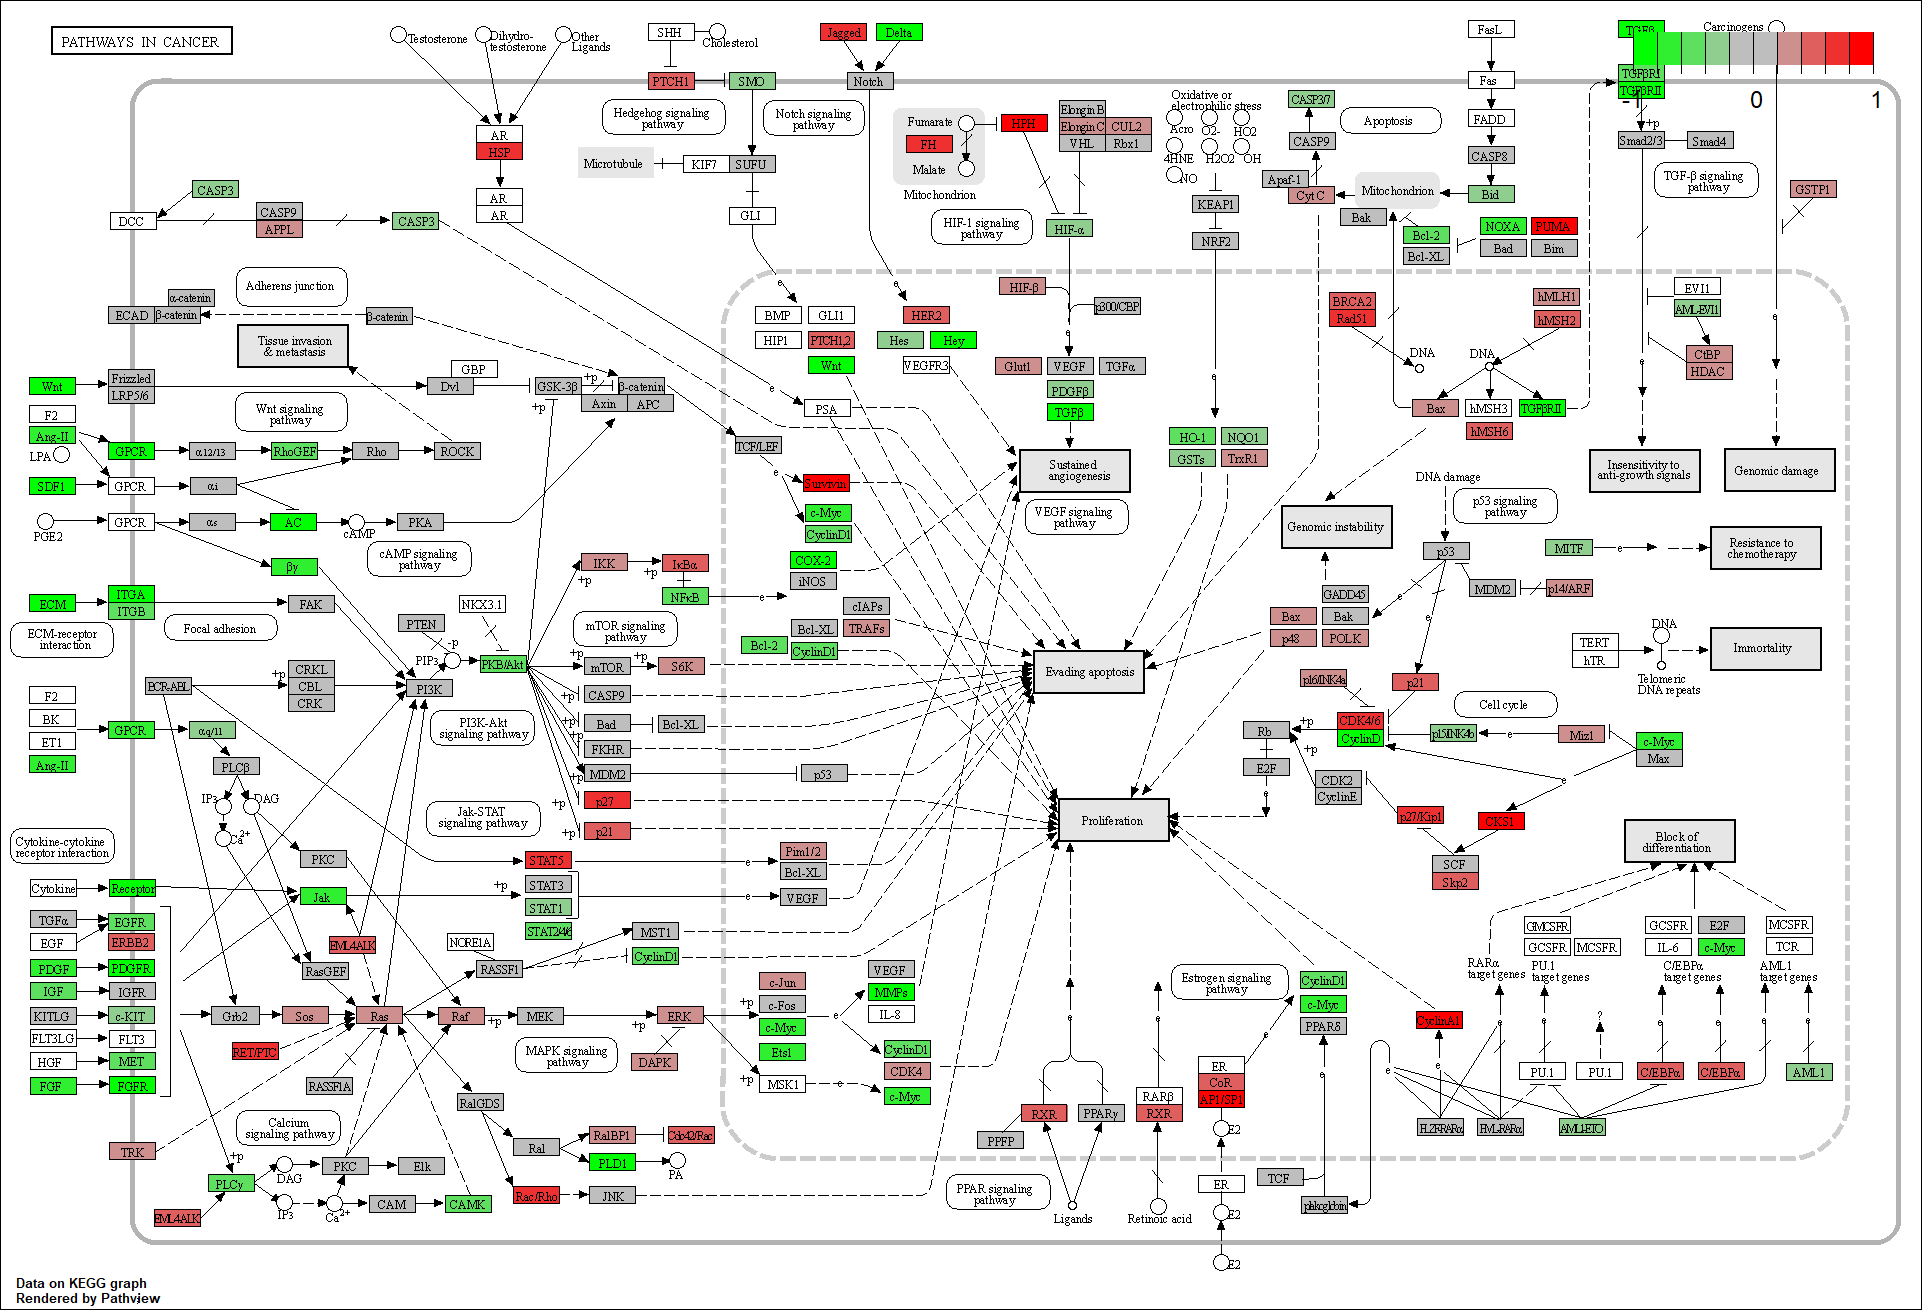
\includegraphics{Figs/mmu05200.ComDim.png}

\hypertarget{Section6}{%
\chapter{Data from a single omics data are multi-blocks}\label{Section6}}

In the previous sections, we have only used \textbf{ComDim-PCA}, but many other
ComDim versions exist. ComDim can be regarded as a chemometric method able to
compact the relevant information of the data into a reduced subspace, defined by
the \textbf{scores}, the \textbf{loadings} and the \textbf{saliences}.
Although most ComDim analyses employ \textbf{Principal Component Analysis (PCA)} as
the core method to find this reduced space, other approaches can be used.

The \texttt{R.Comdim} package includes a few of those other methods, as well as some
additional functions \textbf{to allow the users to create their own ComDim methods}.

\hypertarget{PLS}{%
\section{ComDim-Partial Least Squares (ComDim-PLS)}\label{PLS}}

\begin{Shaded}
\begin{Highlighting}[]
\NormalTok{resultsPLSR }\OtherTok{\textless{}{-}} \FunctionTok{ComDim\_PLS\_MB}\NormalTok{(allMB,}
                             \AttributeTok{y=} \FunctionTok{c}\NormalTok{(}\FunctionTok{rep}\NormalTok{(}\DecValTok{1}\NormalTok{,}\DecValTok{4}\NormalTok{),}\FunctionTok{rep}\NormalTok{(}\DecValTok{5}\NormalTok{,}\DecValTok{4}\NormalTok{),}\FunctionTok{rep}\NormalTok{(}\DecValTok{10}\NormalTok{,}\DecValTok{4}\NormalTok{)),}
                             \CommentTok{\# Arbitrary scale, just for the demonstration}
                             \AttributeTok{ndim =} \DecValTok{2}\NormalTok{, }\AttributeTok{method =} \StringTok{\textquotesingle{}PLS{-}R\textquotesingle{}}\NormalTok{)}
\end{Highlighting}
\end{Shaded}

\hypertarget{PLS-DA}{%
\section{ComDim-Partial Least Squares Discriminant Analysis (ComDim-PLSDA)}\label{PLS-DA}}

\begin{Shaded}
\begin{Highlighting}[]
\NormalTok{resultsPLSDA }\OtherTok{\textless{}{-}} \FunctionTok{ComDim\_PLS\_MB}\NormalTok{(allMB,}
                              \AttributeTok{y=} \FunctionTok{c}\NormalTok{(}\FunctionTok{rep}\NormalTok{(}\StringTok{\textquotesingle{}NI\textquotesingle{}}\NormalTok{,}\DecValTok{4}\NormalTok{),}\FunctionTok{rep}\NormalTok{(}\StringTok{\textquotesingle{}DOX\textquotesingle{}}\NormalTok{,}\DecValTok{4}\NormalTok{),}\FunctionTok{rep}\NormalTok{(}\StringTok{\textquotesingle{}OFF\textquotesingle{}}\NormalTok{,}\DecValTok{4}\NormalTok{)),}
                              \AttributeTok{ndim =} \DecValTok{2}\NormalTok{, }\AttributeTok{method =} \StringTok{\textquotesingle{}PLS{-}DA\textquotesingle{}}\NormalTok{)}

\CommentTok{\# Method evaluation}
\NormalTok{resultsPLSDA}\SpecialCharTok{@}\NormalTok{R2X}
\NormalTok{resultsPLSDA}\SpecialCharTok{@}\NormalTok{R2Y}
\NormalTok{resultsPLSDA}\SpecialCharTok{@}\NormalTok{Q2}
\NormalTok{resultsPLSDA}\SpecialCharTok{@}\NormalTok{Prediction}\SpecialCharTok{$}\NormalTok{confusionMatrix}

\CommentTok{\# Plot saliences}
\NormalTok{saliencesPLSDA }\OtherTok{\textless{}{-}}\NormalTok{ resultsPLSDA}\SpecialCharTok{@}\NormalTok{Saliences }\SpecialCharTok{\%\textgreater{}\%}
  \FunctionTok{as.data.frame}\NormalTok{() }\SpecialCharTok{\%\textgreater{}\%}
  \FunctionTok{mutate}\NormalTok{(}\AttributeTok{dataset =} \FunctionTok{rownames}\NormalTok{(.)) }\SpecialCharTok{\%\textgreater{}\%}
  \FunctionTok{pivot\_longer}\NormalTok{(}\AttributeTok{cols =} \FunctionTok{c}\NormalTok{(}\StringTok{\textquotesingle{}CC1\textquotesingle{}}\NormalTok{,}\StringTok{\textquotesingle{}CC2\textquotesingle{}}\NormalTok{),}
               \AttributeTok{names\_to =} \StringTok{\textquotesingle{}CC\textquotesingle{}}\NormalTok{,}
               \AttributeTok{values\_to =} \StringTok{\textquotesingle{}Salience\textquotesingle{}}\NormalTok{)}

\FunctionTok{ggplot}\NormalTok{(}\AttributeTok{data =}\NormalTok{ saliencesPLSDA,}
       \FunctionTok{aes}\NormalTok{(}\AttributeTok{x =}\NormalTok{ CC, }\AttributeTok{y =}\NormalTok{ Salience, }\AttributeTok{group =}\NormalTok{ dataset )) }\SpecialCharTok{+}
  \FunctionTok{geom\_bar}\NormalTok{(}\AttributeTok{stat =} \StringTok{\textquotesingle{}identity\textquotesingle{}}\NormalTok{, }\AttributeTok{position =} \StringTok{\textquotesingle{}dodge\textquotesingle{}}\NormalTok{,}
           \FunctionTok{aes}\NormalTok{(}\AttributeTok{fill =}\NormalTok{ dataset)) }\SpecialCharTok{+}
  \FunctionTok{theme\_minimal}\NormalTok{() }\SpecialCharTok{+}
  \FunctionTok{labs}\NormalTok{(}\AttributeTok{title =} \StringTok{\textquotesingle{}ComDim Saliences\textquotesingle{}}\NormalTok{)}

\CommentTok{\# Plot scores}
\NormalTok{scoresTable }\OtherTok{\textless{}{-}} \FunctionTok{MakeComDimScoresTable}\NormalTok{(}\AttributeTok{model =}\NormalTok{ resultsPLSDA)}
\NormalTok{scoresTable\_wider }\OtherTok{\textless{}{-}}\NormalTok{ scoresTable }\SpecialCharTok{\%\textgreater{}\%}
  \FunctionTok{mutate}\NormalTok{(}\AttributeTok{sample.type =} \FunctionTok{case\_when}\NormalTok{(}\FunctionTok{grepl}\NormalTok{(}\StringTok{\textquotesingle{}DOX\textquotesingle{}}\NormalTok{, sample.id) }\SpecialCharTok{\textasciitilde{}} \StringTok{\textquotesingle{}DOX\textquotesingle{}}\NormalTok{,}
                                 \FunctionTok{grepl}\NormalTok{(}\StringTok{\textquotesingle{}NI\textquotesingle{}}\NormalTok{, sample.id) }\SpecialCharTok{\textasciitilde{}} \StringTok{\textquotesingle{}NI\textquotesingle{}}\NormalTok{,}
                                 \FunctionTok{grepl}\NormalTok{(}\StringTok{\textquotesingle{}OFF\textquotesingle{}}\NormalTok{, sample.id) }\SpecialCharTok{\textasciitilde{}} \StringTok{\textquotesingle{}OFF\textquotesingle{}}\NormalTok{)) }\SpecialCharTok{\%\textgreater{}\%}
\NormalTok{  dplyr}\SpecialCharTok{::}\FunctionTok{select}\NormalTok{(sample.id, sample.type, block.name, scores.type.dim, value) }\SpecialCharTok{\%\textgreater{}\%}
\NormalTok{  dplyr}\SpecialCharTok{::}\FunctionTok{group\_by}\NormalTok{(sample.id, sample.type, scores.type.dim, block.name) }\SpecialCharTok{\%\textgreater{}\%}
  \FunctionTok{pivot\_wider}\NormalTok{(}\AttributeTok{names\_from =}\NormalTok{ scores.type.dim, }\AttributeTok{values\_from =}\NormalTok{ value)}

\FunctionTok{ggplot}\NormalTok{(}\AttributeTok{data =}\NormalTok{ scoresTable\_wider) }\SpecialCharTok{+}
  \FunctionTok{geom\_point}\NormalTok{(}\FunctionTok{aes}\NormalTok{(}\AttributeTok{x =}\NormalTok{ T.scores1, }\AttributeTok{y =}\NormalTok{ T.scores2,}
                 \AttributeTok{color =}\NormalTok{ sample.type, }\AttributeTok{shape =}\NormalTok{ block.name)) }\SpecialCharTok{+}
  \FunctionTok{geom\_point}\NormalTok{(}\FunctionTok{aes}\NormalTok{(}\AttributeTok{x =}\NormalTok{ Q.scores1, }\AttributeTok{y =}\NormalTok{ Q.scores2,}
                 \AttributeTok{fill =}\NormalTok{ sample.type, }\AttributeTok{shape =}\NormalTok{ block.name),}
             \AttributeTok{size =} \DecValTok{3}\NormalTok{, }\AttributeTok{shape =} \DecValTok{24}\NormalTok{, }\AttributeTok{color =} \StringTok{\textquotesingle{}black\textquotesingle{}}\NormalTok{) }\SpecialCharTok{+}
  \FunctionTok{theme\_minimal}\NormalTok{() }\SpecialCharTok{+}
  \FunctionTok{labs}\NormalTok{(}\AttributeTok{title =} \StringTok{\textquotesingle{}ComDim scores {-} PLSDA\textquotesingle{}}\NormalTok{, }\AttributeTok{x =} \StringTok{\textquotesingle{}CC1\textquotesingle{}}\NormalTok{, }\AttributeTok{y =} \StringTok{\textquotesingle{}CC2\textquotesingle{}}\NormalTok{)}
\end{Highlighting}
\end{Shaded}

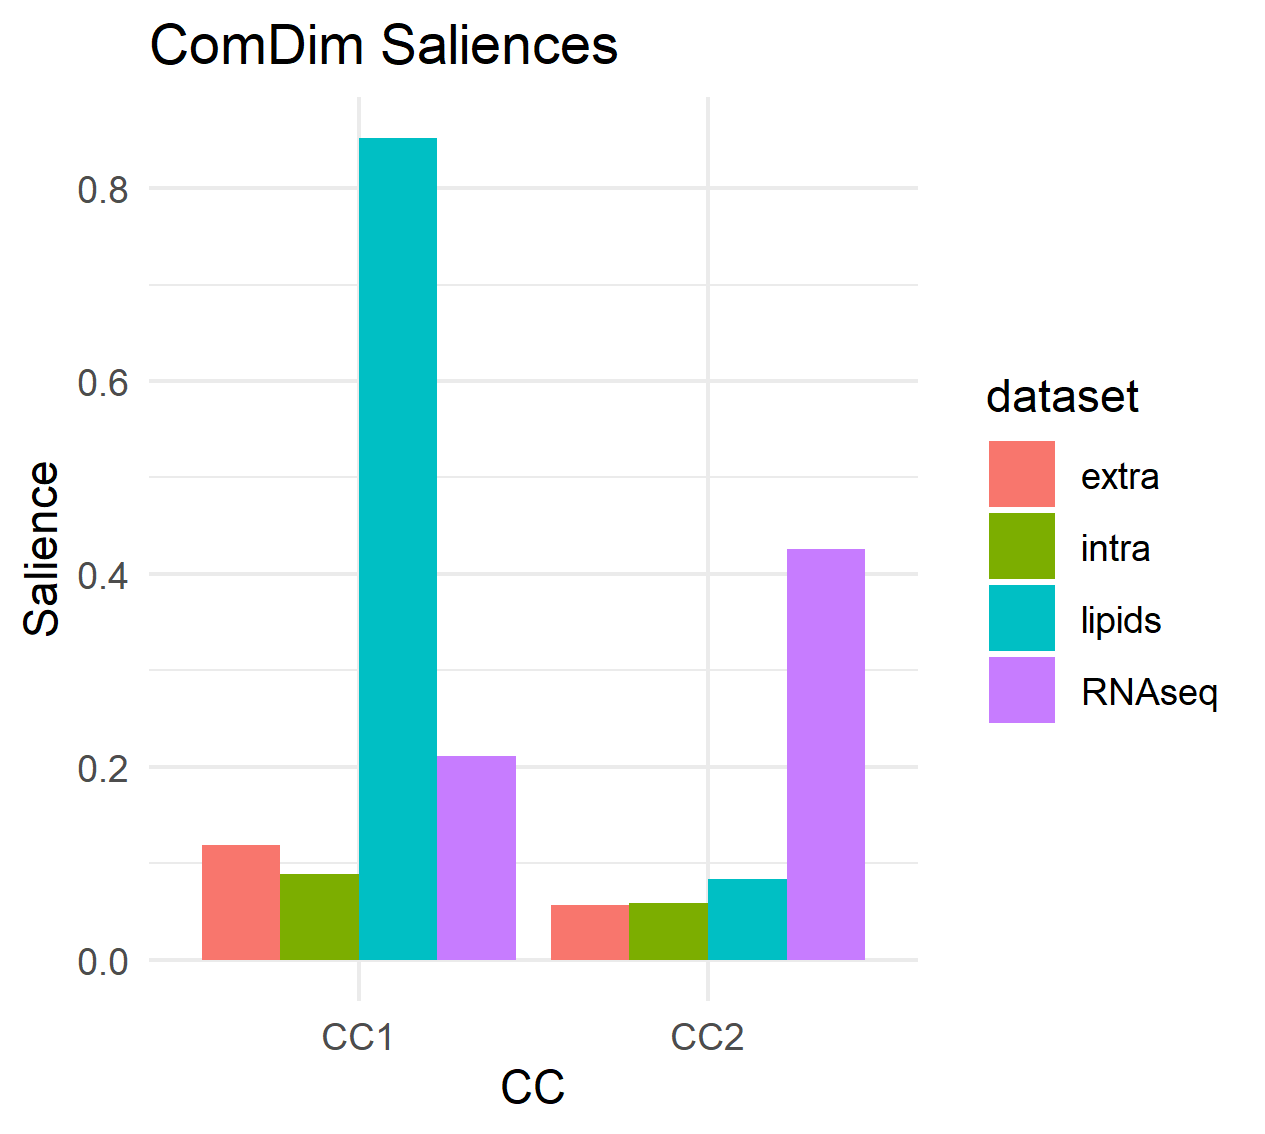
\includegraphics{Figs/fig6_1.png}
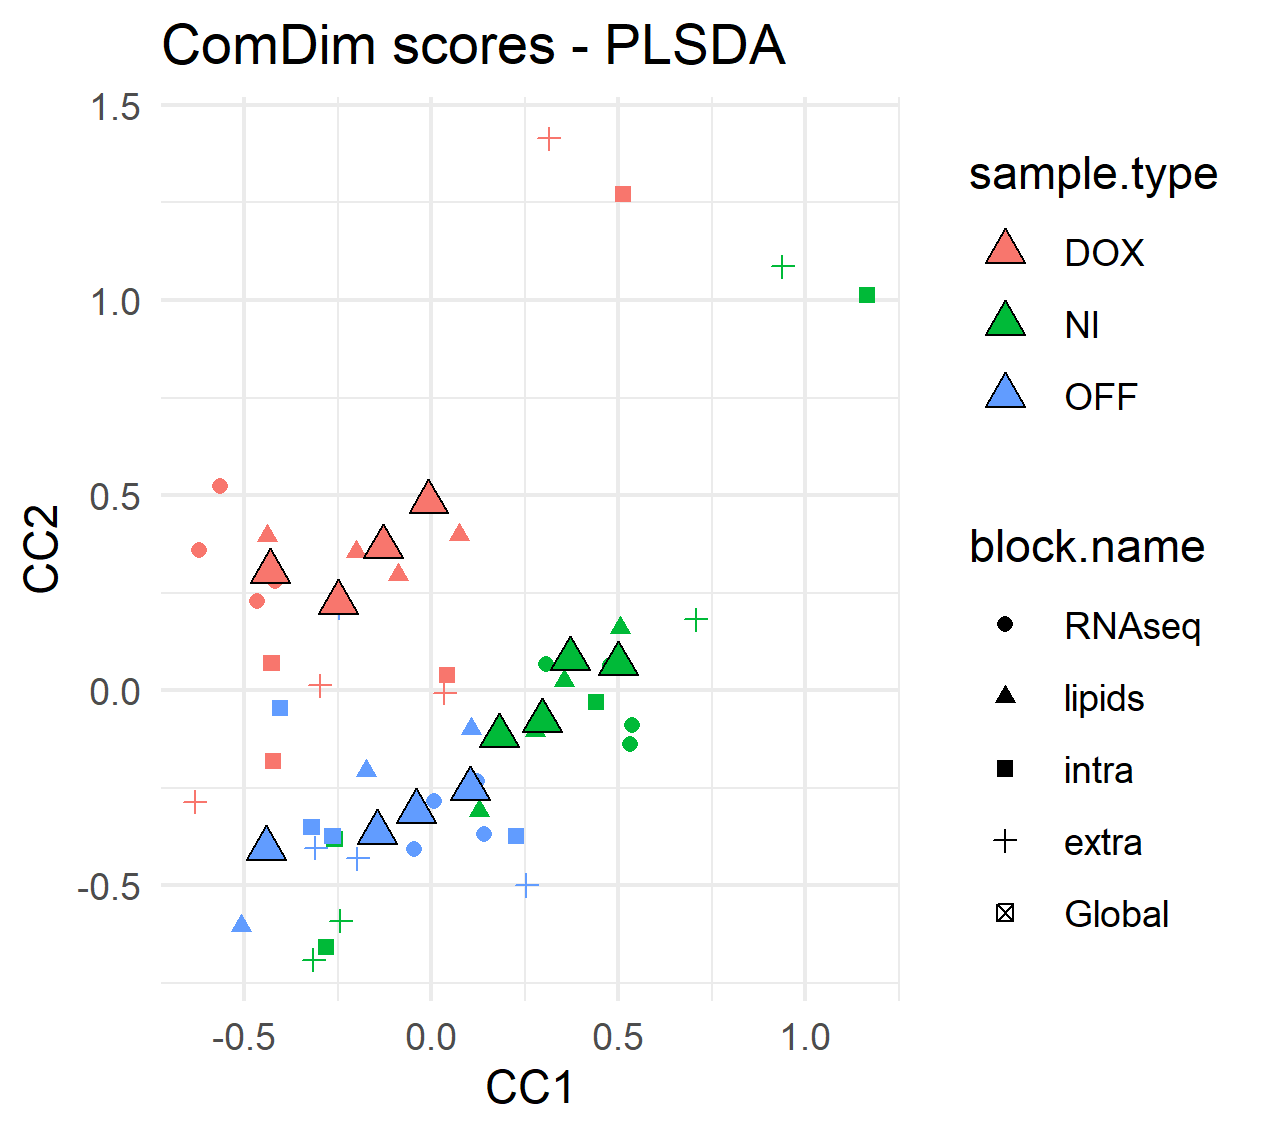
\includegraphics{Figs/fig6_2.png}

\hypertarget{KOPLS}{%
\section{ComDim-kernel-OPLS}\label{KOPLS}}

\begin{Shaded}
\begin{Highlighting}[]
\FunctionTok{source}\NormalTok{(}\StringTok{\textquotesingle{}./R/ComDim\_KOPLS\_MB.R\textquotesingle{}}\NormalTok{)}
\NormalTok{resultsKOPLSDA }\OtherTok{\textless{}{-}} \FunctionTok{ComDim\_KOPLS\_MB}\NormalTok{(allMB, }\AttributeTok{y=} \FunctionTok{c}\NormalTok{(}\FunctionTok{rep}\NormalTok{(}\StringTok{\textquotesingle{}NI\textquotesingle{}}\NormalTok{,}\DecValTok{4}\NormalTok{),}\FunctionTok{rep}\NormalTok{(}\StringTok{\textquotesingle{}DOX\textquotesingle{}}\NormalTok{,}\DecValTok{4}\NormalTok{),}\FunctionTok{rep}\NormalTok{(}\StringTok{\textquotesingle{}OFF\textquotesingle{}}\NormalTok{,}\DecValTok{4}\NormalTok{)),}
                                  \AttributeTok{max.ort =} \DecValTok{2}\NormalTok{, }\AttributeTok{method =} \StringTok{\textquotesingle{}k{-}OPLS{-}DA\textquotesingle{}}\NormalTok{, }\AttributeTok{nrcv =} \DecValTok{5}\NormalTok{)}
\end{Highlighting}
\end{Shaded}

\hypertarget{Other}{%
\section{Other extensions}\label{Other}}

The functions \texttt{ComDim\_Exploratory\_MB()} and \texttt{ComDim\_y\_MB()} can be employed to
use customized versions of Com-Dim for exploratory and regression/discriminant
purposes. In both functions, the parameter \texttt{FUN} allows the user to run ComDim
with their chemometric method of preference.

\hypertarget{example-of-comdim-ica}{%
\subsection{Example of ComDim-ICA}\label{example-of-comdim-ica}}

The function used to execute \textbf{Independent Component Analysis (ICA)} was
\texttt{ica()} from the \texttt{ica} package.
In order to make the \texttt{ComDim\_Exploratory\_MB()} function to understand the output
of \texttt{ica()}, we embedded it into another function that returns the source
estimates (representative of the samples information, analogous to the PCA
scores) named \texttt{fun.ICA}.

\begin{Shaded}
\begin{Highlighting}[]
\FunctionTok{library}\NormalTok{(ica)}

\NormalTok{fun.ICA }\OtherTok{\textless{}{-}} \ControlFlowTok{function}\NormalTok{(W, ndim,...)\{}
  \CommentTok{\# W is the concatenated MB.}
  \CommentTok{\# ndim is the number of components.}
  \CommentTok{\# X and nc are the arguments of ica::ica.}
\NormalTok{  result }\OtherTok{\textless{}{-}}\NormalTok{ ica}\SpecialCharTok{::}\FunctionTok{ica}\NormalTok{(W, ndim)}
\NormalTok{  sources }\OtherTok{\textless{}{-}}\NormalTok{ result}\SpecialCharTok{$}\NormalTok{S}
  \CommentTok{\# The function must return the source estimates}
  \CommentTok{\# The analogue to the PCA scores for ICA.}
  \FunctionTok{return}\NormalTok{(sources)}
\NormalTok{\}}
\NormalTok{resultsICA }\OtherTok{\textless{}{-}} \FunctionTok{ComDim\_Exploratory\_MB}\NormalTok{(allMB, }\AttributeTok{ndim =} \DecValTok{2}\NormalTok{,}
                                    \AttributeTok{FUN =}\NormalTok{ fun.ICA,}
                                    \AttributeTok{method =} \StringTok{\textquotesingle{}ICA\textquotesingle{}}\NormalTok{)}
\end{Highlighting}
\end{Shaded}

\hypertarget{example-of-comdim-pls-version-ropls}{%
\subsection{Example of ComDim-PLS (version ropls)}\label{example-of-comdim-pls-version-ropls}}

The function used to execute \textbf{PLS} here was \texttt{opls()}, obtained from the
\texttt{ropls} package.
In this case, \texttt{fun.PLS} is used to capture the output from the PLS analysis
(scores,P,W,U,Q,y).

\begin{Shaded}
\begin{Highlighting}[]
\FunctionTok{library}\NormalTok{(ropls) }\CommentTok{\# From bioconductor}
\FunctionTok{source}\NormalTok{(}\StringTok{\textquotesingle{}./R/ComDim\_y\_MB.R\textquotesingle{}}\NormalTok{)}
\NormalTok{fun.PLS }\OtherTok{\textless{}{-}} \ControlFlowTok{function}\NormalTok{(W, y, ndim,...)\{}
  \CommentTok{\# W is the concatenated MB.}
  \CommentTok{\# ndim is the number of components.}
  \CommentTok{\# X and nc are the arguments of ica::ica.}
\NormalTok{  output }\OtherTok{\textless{}{-}} \FunctionTok{list}\NormalTok{()}
\NormalTok{  result }\OtherTok{\textless{}{-}}\NormalTok{ ropls}\SpecialCharTok{::}\FunctionTok{opls}\NormalTok{(}\AttributeTok{x =}\NormalTok{ W, }\AttributeTok{y =}\NormalTok{ y, }\AttributeTok{predI =}\NormalTok{ ndim,}
                        \AttributeTok{fig.pdfC =} \StringTok{\textquotesingle{}none\textquotesingle{}}\NormalTok{,}
                        \AttributeTok{info.txtC =} \StringTok{\textquotesingle{}none\textquotesingle{}}\NormalTok{)}
  \CommentTok{\# The returning object must be a list containing the following 6 elements:}
\NormalTok{  output}\SpecialCharTok{$}\NormalTok{scores }\OtherTok{\textless{}{-}}\NormalTok{ result}\SpecialCharTok{@}\NormalTok{scoreMN[,}\DecValTok{1}\NormalTok{]}
\NormalTok{  output}\SpecialCharTok{$}\NormalTok{P }\OtherTok{\textless{}{-}}\NormalTok{ result}\SpecialCharTok{@}\NormalTok{loadingMN[,}\DecValTok{1}\NormalTok{]}
\NormalTok{  output}\SpecialCharTok{$}\NormalTok{W }\OtherTok{\textless{}{-}}\NormalTok{ result}\SpecialCharTok{@}\NormalTok{weightMN[,}\DecValTok{1}\NormalTok{]}
\NormalTok{  output}\SpecialCharTok{$}\NormalTok{U }\OtherTok{\textless{}{-}}\NormalTok{ result}\SpecialCharTok{@}\NormalTok{uMN[,}\DecValTok{1}\NormalTok{]}
\NormalTok{  output}\SpecialCharTok{$}\NormalTok{Q }\OtherTok{\textless{}{-}}\NormalTok{ result}\SpecialCharTok{@}\NormalTok{cMN[,}\DecValTok{1}\NormalTok{]}
\NormalTok{  output}\SpecialCharTok{$}\NormalTok{y }\OtherTok{\textless{}{-}}\NormalTok{ result}\SpecialCharTok{@}\NormalTok{suppLs}\SpecialCharTok{$}\NormalTok{yModelMN }\CommentTok{\# To evaluate if y is transformed within opls. (it is!)}
  \FunctionTok{return}\NormalTok{(output)}
\NormalTok{\}}
\NormalTok{resultsPLS }\OtherTok{\textless{}{-}} \FunctionTok{ComDim\_y\_MB}\NormalTok{(allMB,}
                          \AttributeTok{y =}\FunctionTok{c}\NormalTok{(}\FunctionTok{rep}\NormalTok{(}\DecValTok{1}\NormalTok{,}\DecValTok{4}\NormalTok{),}\FunctionTok{rep}\NormalTok{(}\DecValTok{5}\NormalTok{,}\DecValTok{4}\NormalTok{),}\FunctionTok{rep}\NormalTok{(}\DecValTok{10}\NormalTok{,}\DecValTok{4}\NormalTok{)),}
                          \AttributeTok{ndim =} \DecValTok{2}\NormalTok{,}
                          \AttributeTok{type =} \StringTok{\textquotesingle{}regression\textquotesingle{}}\NormalTok{,}
                          \AttributeTok{orthogonalization =} \ConstantTok{FALSE}\NormalTok{,}
                          \AttributeTok{FUN =}\NormalTok{ fun.PLS,}
                          \AttributeTok{method =} \StringTok{\textquotesingle{}PLS(ropls)\textquotesingle{}}\NormalTok{)}
\end{Highlighting}
\end{Shaded}

\hypertarget{example-of-comdim-plsda-version-ropls}{%
\subsection{Example of ComDim-PLSDA (version ropls)}\label{example-of-comdim-plsda-version-ropls}}

For ComDim-PLS-DA, we can use the same function \texttt{fun.PLS} as before, but we need
to specify that the \texttt{type} of the method is \texttt{\textquotesingle{}discriminant\textquotesingle{}} and we need to
provide the sample classes in \texttt{y}:

\begin{Shaded}
\begin{Highlighting}[]
\NormalTok{resultsPLSDA }\OtherTok{\textless{}{-}} \FunctionTok{ComDim\_y\_MB}\NormalTok{(allMB,}
                           \AttributeTok{y =}\FunctionTok{c}\NormalTok{(}\FunctionTok{rep}\NormalTok{(}\StringTok{\textquotesingle{}NI\textquotesingle{}}\NormalTok{,}\DecValTok{4}\NormalTok{),}\FunctionTok{rep}\NormalTok{(}\StringTok{\textquotesingle{}DOX\textquotesingle{}}\NormalTok{,}\DecValTok{4}\NormalTok{),}\FunctionTok{rep}\NormalTok{(}\StringTok{\textquotesingle{}OFF\textquotesingle{}}\NormalTok{,}\DecValTok{4}\NormalTok{)),}
                           \AttributeTok{ndim =} \DecValTok{2}\NormalTok{,}
                           \AttributeTok{type =} \StringTok{\textquotesingle{}discriminant\textquotesingle{}}\NormalTok{,}
                           \AttributeTok{orthogonalization =} \ConstantTok{FALSE}\NormalTok{,}
                           \AttributeTok{FUN =}\NormalTok{ fun.PLS,}
                           \AttributeTok{method =} \StringTok{\textquotesingle{}PLSDA(ropls)\textquotesingle{}}\NormalTok{)}
\end{Highlighting}
\end{Shaded}

\hypertarget{example-of-comdim-oplsda-version-ropls}{%
\subsection{Example of ComDim-OPLSDA (version ropls)}\label{example-of-comdim-oplsda-version-ropls}}

For ComDim-OPLSDA, the function in \texttt{FUN} needs to capture additional outputs
related to the orthogonal components. See the example below:

\begin{Shaded}
\begin{Highlighting}[]
\CommentTok{\# We will apply ComDim{-}OPLSDA on a subset with 2 classes only.}
\NormalTok{allMB\_small }\OtherTok{\textless{}{-}} \FunctionTok{FilterSamples\_MB}\NormalTok{(allMB,}
                                \FunctionTok{getSampleNames}\NormalTok{(allMB)[}\FunctionTok{c}\NormalTok{(}\DecValTok{1}\SpecialCharTok{:}\DecValTok{4}\NormalTok{,}\DecValTok{9}\SpecialCharTok{:}\DecValTok{12}\NormalTok{)])}
\NormalTok{fun.OPLSDA }\OtherTok{\textless{}{-}} \ControlFlowTok{function}\NormalTok{(W, y, ndim,...)\{}
  \CommentTok{\# W is the concatenated MB.}
  \CommentTok{\# ndim is the number of components.}
\NormalTok{  output }\OtherTok{\textless{}{-}} \FunctionTok{list}\NormalTok{()}
\NormalTok{  Y }\OtherTok{\textless{}{-}} \FunctionTok{c}\NormalTok{(}\SpecialCharTok{{-}}\DecValTok{1}\NormalTok{,}\DecValTok{1}\NormalTok{)[}\FunctionTok{apply}\NormalTok{(y, }\DecValTok{1}\NormalTok{, }\ControlFlowTok{function}\NormalTok{(x) }\FunctionTok{match}\NormalTok{(}\DecValTok{1}\NormalTok{,x))]}
  \CommentTok{\# Y must be a vector for ropls}
\NormalTok{  result }\OtherTok{\textless{}{-}}\NormalTok{ ropls}\SpecialCharTok{::}\FunctionTok{opls}\NormalTok{(}\AttributeTok{x =}\NormalTok{ W, }\AttributeTok{y =}\NormalTok{ Y,}
                        \AttributeTok{predI =} \DecValTok{1}\NormalTok{,}
                        \AttributeTok{orthoI =} \ConstantTok{NA}\NormalTok{, }\CommentTok{\# The number of orthogonal components}
                                     \CommentTok{\# is optimized for every block.}
                        \AttributeTok{fig.pdfC =} \StringTok{\textquotesingle{}none\textquotesingle{}}\NormalTok{,}
                        \AttributeTok{info.txtC =} \StringTok{\textquotesingle{}none\textquotesingle{}}\NormalTok{)}
  \CommentTok{\# The returning object must be a list containing the following 9 elements:}
\NormalTok{  output}\SpecialCharTok{$}\NormalTok{scores }\OtherTok{\textless{}{-}}\NormalTok{ result}\SpecialCharTok{@}\NormalTok{scoreMN[,}\DecValTok{1}\NormalTok{]}
\NormalTok{  output}\SpecialCharTok{$}\NormalTok{P }\OtherTok{\textless{}{-}}\NormalTok{ result}\SpecialCharTok{@}\NormalTok{loadingMN[,}\DecValTok{1}\NormalTok{]}
\NormalTok{  output}\SpecialCharTok{$}\NormalTok{W }\OtherTok{\textless{}{-}}\NormalTok{ result}\SpecialCharTok{@}\NormalTok{weightMN[,}\DecValTok{1}\NormalTok{]}
\NormalTok{  output}\SpecialCharTok{$}\NormalTok{U }\OtherTok{\textless{}{-}}\NormalTok{ result}\SpecialCharTok{@}\NormalTok{uMN[,}\DecValTok{1}\NormalTok{]}
\NormalTok{  output}\SpecialCharTok{$}\NormalTok{Q }\OtherTok{\textless{}{-}}\NormalTok{ result}\SpecialCharTok{@}\NormalTok{cMN[,}\DecValTok{1}\NormalTok{]}
\NormalTok{  output}\SpecialCharTok{$}\NormalTok{Q }\OtherTok{\textless{}{-}} \FunctionTok{c}\NormalTok{(}\SpecialCharTok{{-}}\NormalTok{output}\SpecialCharTok{$}\NormalTok{Q,output}\SpecialCharTok{$}\NormalTok{Q)}
  \CommentTok{\# Y has two columns (one per class): {-}1 and 1.}
\NormalTok{  output}\SpecialCharTok{$}\NormalTok{y }\OtherTok{\textless{}{-}}\NormalTok{ result}\SpecialCharTok{@}\NormalTok{suppLs}\SpecialCharTok{$}\NormalTok{yModelMN}
  \CommentTok{\# To evaluate if y is transformed within opls. (it is!)}
\NormalTok{  output}\SpecialCharTok{$}\NormalTok{orthoscores }\OtherTok{\textless{}{-}}\NormalTok{ result}\SpecialCharTok{@}\NormalTok{orthoScoreMN}
\NormalTok{  output}\SpecialCharTok{$}\NormalTok{orthoP }\OtherTok{\textless{}{-}}\NormalTok{ result}\SpecialCharTok{@}\NormalTok{orthoLoadingMN}
\NormalTok{  output}\SpecialCharTok{$}\NormalTok{ort }\OtherTok{\textless{}{-}}\NormalTok{ result}\SpecialCharTok{@}\NormalTok{summaryDF}\SpecialCharTok{$}\NormalTok{ort }\CommentTok{\# Number of orthogonal components}
  \FunctionTok{return}\NormalTok{(output)}
\NormalTok{\}}
\NormalTok{resultsOPLSDA }\OtherTok{\textless{}{-}} \FunctionTok{ComDim\_y\_MB}\NormalTok{(allMB\_small,}
                            \AttributeTok{y =}\FunctionTok{c}\NormalTok{(}\FunctionTok{rep}\NormalTok{(}\StringTok{\textquotesingle{}NI\textquotesingle{}}\NormalTok{,}\DecValTok{4}\NormalTok{),}\FunctionTok{rep}\NormalTok{(}\StringTok{\textquotesingle{}OFF\textquotesingle{}}\NormalTok{,}\DecValTok{4}\NormalTok{)),}
                            \AttributeTok{ndim =} \DecValTok{1}\NormalTok{,}
                            \AttributeTok{type =} \StringTok{\textquotesingle{}discriminant\textquotesingle{}}\NormalTok{,}
                            \AttributeTok{orthogonalization =} \ConstantTok{TRUE}\NormalTok{,}
                            \AttributeTok{FUN =}\NormalTok{ fun.OPLSDA,}
                            \AttributeTok{method =} \StringTok{\textquotesingle{}OPLSDA(ropls)\textquotesingle{}}\NormalTok{)}
\end{Highlighting}
\end{Shaded}


  \bibliography{book.bib,packages.bib}

\end{document}
